\section{Constitutive models}
\label{sec:constitutive}
\index{constitutiveModels}
\index{Constitutive block}
\index{MPM constitutive dispatch}

This section documents the continuum constitutive models used by the MPM solver.  Cohesive-zone material laws are documented separately in Section~\ref{sec:cohesive-zone-implementation}, because they operate on interface opening/sliding states rather than on ordinary particle volume states.  The continuum models described here are defined in the XML \texttt{Constitutive} block and assigned to particles through \texttt{ParticleRegion} material lists.  PFW assigns the particle material index as described in Section~\ref{sec:pfw-materials}; during the explicit step, that index selects the GEOS constitutive object used at Step~16, Section~\ref{subsec:solver-step-16}.

For a continuum particle, the solver supplies the material update with the current or incremental kinematic state, density, volume, temperature, porosity, damage, material direction, and any model-specific history fields.  The constitutive model returns the updated Cauchy stress, updated history variables, material wave-speed data used by the CFL estimate, and a constitutive update flag that may be consumed by the robustness controls in Section~\ref{sec:robustness-controls}.  The common notation used below is
\begin{align}
  \mathbf{F}_{p}^{n+1} &= \text{deformation gradient},
  & J_p &= \det \mathbf{F}_{p}^{n+1}, \\
  \Delta \boldsymbol{\epsilon}_p &= \text{corotational strain increment},
  & \mathbf{D}_p &= \frac{1}{2}\left(\mathbf{L}_p+\mathbf{L}_p^T\right), \\
  p &= -\frac{1}{3}\operatorname{tr}\boldsymbol{\sigma},
  & \mathbf{s} &= \boldsymbol{\sigma}+p\mathbf{I},
  & q &= \sqrt{\frac{3}{2}\mathbf{s}:\mathbf{s}} .
\end{align}
The sign convention is the GEOS stress convention used by the material implementation; the equations below are written to expose the algorithmic structure rather than to replace the source code for calibration.

\subsection{Solid models}
\label{subsec:solid-constitutive-models}
\index{constitutiveModels!solid models}

The MPM-connected solid models share a common explicit-update skeleton.  Depending on the model, the update may be a small-strain corotational update, a finite-deformation hyperelastic update based directly on \(\mathbf{F}\), or an elastic predictor followed by an inelastic/damage corrector.  The following algorithm is the common solver-side pattern; individual models replace the \texttt{materialUpdate} line with the specialized laws described in the following subsections.

\begin{lstlisting}[caption={Common explicit MPM continuum material update pattern.},label={alg:continuum-material-dispatch},basicstyle=\ttfamily\small]
for active particle p:
  read material index mat[p]
  gather F[p], J[p], strainIncrement[p], velocityGradient[p]
  gather optional fields: temperature, porosity, damage,
                          strengthScale, materialDirection,
                          distanceToCrackTip
  (stress[p], state[p], waveSpeed[p], updateFlag[p]) =
      materialUpdate(mat[p], stressOld[p], stateOld[p], kinematics[p])
  store stress[p] and state[p]
\end{lstlisting}

\subsubsection{\texttt{ElasticIsotropic}}
\label{subsubsec:elastic-isotropic-model}
\index{constitutiveModels!ElasticIsotropic}

\texttt{ElasticIsotropic} is the baseline small-strain isotropic elastic material.  It is useful for mapping tests, wave-speed verification, contact/boundary tests, and reference calculations when the material deformation is small enough that a corotational elastic increment is adequate.  The model is the standard Hooke law form documented in continuum mechanics texts such as Malvern~\cite{malvern1969}.

With bulk modulus \(K\), shear modulus \(G\), and strain increment \(\Delta\boldsymbol{\epsilon}\), the update is
\begin{equation}
  \boldsymbol{\sigma}^{n+1}
  = \boldsymbol{\sigma}^{n}
  + K\operatorname{tr}(\Delta\boldsymbol{\epsilon})\mathbf{I}
  + 2G\operatorname{dev}(\Delta\boldsymbol{\epsilon}).
  \label{eq:elastic-isotropic-update}
\end{equation}
The wave speed used in explicit time-step estimation is the compressional elastic speed
\begin{equation}
  c = \sqrt{\frac{K+4G/3}{\rho}} .
  \label{eq:elastic-isotropic-wavespeed}
\end{equation}

\begin{lstlisting}[caption={ElasticIsotropic stress update.},label={alg:elastic-isotropic-update},basicstyle=\ttfamily\small]
trde = trace(strainIncrement)
devde = strainIncrement - trde/3 * I
stress = oldStress + K * trde * I + 2 * G * devde
waveSpeed = sqrt((K + 4*G/3) / density)
\end{lstlisting}

\subsubsection{\texttt{Hyperelastic}}
\label{subsubsec:hyperelastic-model}
\index{constitutiveModels!Hyperelastic}

\texttt{Hyperelastic} is the finite-deformation elastic baseline.  It is used when the stress should be evaluated from the deformation gradient instead of from an accumulated infinitesimal strain increment.  The implementation uses an isochoric-volumetric split typical of compressible neo-Hookean finite elasticity~\cite{ogden1997,holzapfel2000}.  Let
\begin{equation}
  \mathbf{B}=\mathbf{F}\mathbf{F}^{T},
  \qquad
  J=\det\mathbf{F},
  \qquad
  \bar{\mathbf{B}}=J^{-2/3}\mathbf{B} .
\end{equation}
The current implementation evaluates the Cauchy stress as
\begin{equation}
  \boldsymbol{\sigma}
  = G J^{-5/3}\mathbf{B}
  + \left[K(J-1)-\frac{G}{3}J^{-5/3}\operatorname{tr}\mathbf{B}\right]\mathbf{I}.
  \label{eq:geos-hyperelastic-stress}
\end{equation}
This form is equivalent to a compressible neo-Hookean-style response with a volumetric penalty and an isochoric deviatoric contribution.  It is a convenient large-deformation elastic model for solver verification, prescribed deformation, and simple contact calculations.

\begin{lstlisting}[caption={Hyperelastic stress update.},label={alg:hyperelastic-update},basicstyle=\ttfamily\small]
F = I + FminusI
B = F * transpose(F)
J = det(F)
x1 = G / J^(5/3)
x2 = K * (J - 1) - G * trace(B) / (3 * J^(5/3))
stress = x1 * B + x2 * I
\end{lstlisting}

\subsubsection{\texttt{HyperelasticMMS}}
\label{subsubsec:hyperelastic-mms-model}
\index{constitutiveModels!HyperelasticMMS}
\index{manufactured solution}

\texttt{HyperelasticMMS} is a manufactured-solution variant of the finite-deformation hyperelastic path.  It should be treated as a verification material rather than as a production constitutive law.  Its purpose is to pair a known analytical displacement/velocity/stress field with body forces and boundary data so that the particle-grid mapping, explicit integration, and boundary treatment can be tested in a controlled setting.  The method of manufactured solutions is a standard code-verification approach~\cite{roache1998}.

The current MMS hyperelastic stress uses
\begin{equation}
  \boldsymbol{\sigma}
  = \frac{\lambda \ln J}{J}\mathbf{I}
  + \frac{G}{J}(\mathbf{B}-\mathbf{I}),
  \label{eq:hyperelastic-mms-stress}
\end{equation}
where \(\lambda\) is the first Lame constant.  Compared with Eq.~\eqref{eq:geos-hyperelastic-stress}, this form is closer to the commonly used compressible neo-Hookean Cauchy stress.

\begin{lstlisting}[caption={HyperelasticMMS stress update.},label={alg:hyperelastic-mms-update},basicstyle=\ttfamily\small]
F = I + FminusI
B = F * transpose(F)
J = det(F)
stress = lambda * log(J) / J * I + G / J * (B - I)
waveSpeed = sqrt((K + 4*G/3) / density)
\end{lstlisting}

\subsubsection{\texttt{ElasticTransverseIsotropic}}
\label{subsubsec:elastic-transverse-isotropic-model}
\index{constitutiveModels!ElasticTransverseIsotropic}
\index{MaterialDirection}

\texttt{ElasticTransverseIsotropic} is the baseline anisotropic elastic solid model.  It represents a material with one preferred axis, such as a fiber direction, bedding normal, crystal axis, or platelet normal.  PFW can assign the particle material basis using \texttt{MaterialDirection}, as described in Section~\ref{sec:pfw-materials}.  The theory follows standard transversely isotropic elasticity~\cite{lekhnitskii1963}.

In the local material frame, the Voigt stiffness is
\begin{equation}
\mathbf{C}_{\mathrm{TI}}=
\begin{bmatrix}
 c_{11} & c_{12} & c_{13} & 0 & 0 & 0 \\
 c_{12} & c_{11} & c_{13} & 0 & 0 & 0 \\
 c_{13} & c_{13} & c_{33} & 0 & 0 & 0 \\
 0 & 0 & 0 & c_{44} & 0 & 0 \\
 0 & 0 & 0 & 0 & c_{44} & 0 \\
 0 & 0 & 0 & 0 & 0 & c_{66}
\end{bmatrix},
\qquad c_{12}=c_{11}-2c_{66}.
\label{eq:ti-stiffness}
\end{equation}
The implementation rotates the local stiffness to the current material direction before applying the strain increment,
\begin{equation}
  \Delta\boldsymbol{\sigma}^{V}=\mathbf{M}(\mathbf{R})\mathbf{C}_{\mathrm{TI}}\mathbf{M}(\mathbf{R})^{T}\Delta\boldsymbol{\epsilon}^{V},
  \label{eq:ti-rotated-stiffness}
\end{equation}
where \(\mathbf{M}(\mathbf{R})\) is the Voigt transformation associated with the rotation from the local transverse-isotropy axis to the particle material direction.

\begin{lstlisting}[caption={Transversely isotropic elastic update.},label={alg:ti-elastic-update},basicstyle=\ttfamily\small]
a = normalize(materialDirection[p])
R = rotation that maps local z-axis to a
M = VoigtRotationMatrix(R)
Cti = localTransverseIsotropicStiffness(c11, c33, c13, c44, c66)
Crot = M * Cti * transpose(M)
stress = oldStress + Crot * strainIncrement
\end{lstlisting}

\subsubsection{\texttt{VonMisesJ}}
\label{subsubsec:von-mises-j-model}
\index{constitutiveModels!VonMisesJ}
\index{J2 plasticity}

\texttt{VonMisesJ} is a pressure-independent \(J_2\) elastoplastic model.  It is appropriate when yielding is controlled primarily by deviatoric stress and a constant yield strength is sufficient.  The implementation computes volumetric response from the deformation-gradient Jacobian, updates deviatoric stress in a corotational frame, and performs a radial return when the von Mises invariant exceeds the yield strength.  This is the standard return-mapping structure for \(J_2\) plasticity~\cite{simo1998inelasticity}.

The yield function is
\begin{equation}
  f(\boldsymbol{\sigma})=q-Y,
  \qquad
  q=\sqrt{\frac{3}{2}\mathbf{s}:\mathbf{s}},
  \label{eq:von-mises-yield}
\end{equation}
where \(Y\) is the current yield strength.  In the current implementation, the pressure-like volumetric part is evaluated from
\begin{equation}
  p = -K\ln J,
  \label{eq:von-mises-volumetric-pressure}
\end{equation}
while the trial deviatoric stress is advanced from the corotational deviatoric rate.  If \(q^{\mathrm{tr}}>Y\), the stress is recomposed with the original trial pressure and the capped deviatoric invariant
\begin{equation}
  \boldsymbol{\sigma}^{n+1}= -p^{\mathrm{tr}}\mathbf{I}
  + \sqrt{\frac{2}{3}}Y\widehat{\mathbf{n}}^{\mathrm{tr}},
  \qquad
  \widehat{\mathbf{n}}^{\mathrm{tr}}=\frac{\mathbf{s}^{\mathrm{tr}}}{\|\mathbf{s}^{\mathrm{tr}}\|}.
\end{equation}

\begin{lstlisting}[caption={VonMisesJ radial-return structure.},label={alg:von-mises-update},basicstyle=\ttfamily\small]
rotate old deviatoric stress to corotational frame
p_trial = -K * log(det(F))
s_trial = old_s + 2 * G * dev(D) * dt
q_trial = sqrt(3/2 * inner(s_trial, s_trial))
if inelasticity disabled or q_trial <= Y:
  stress = -p_trial * I + s_trial
else:
  n_trial = s_trial / norm(s_trial)
  s_returned = sqrt(2/3) * Y * n_trial
  stress = -p_trial * I + s_returned
  update plasticStrain from elastic/plastic strain split
\end{lstlisting}

\subsubsection{\texttt{PerfectlyPlastic}}
\label{subsubsec:perfectly-plastic-model}
\index{constitutiveModels!PerfectlyPlastic}
\index{perfect plasticity}

\texttt{PerfectlyPlastic} is a simpler elastic-perfectly-plastic isotropic model.  It uses the same pressure-independent invariant check as a von Mises material, but does not include hardening.  The elastic predictor is the \texttt{ElasticIsotropic} update.  If the trial stress lies outside the yield surface, the pressure is retained and the deviatoric stress is recomposed with \(q=Y\)~\cite{simo1998inelasticity}.

\begin{equation}
  \boldsymbol{\sigma}^{\mathrm{tr}}
  = \boldsymbol{\sigma}^{n}+K\operatorname{tr}(\Delta\boldsymbol{\epsilon})\mathbf{I}
  +2G\operatorname{dev}(\Delta\boldsymbol{\epsilon}),
  \qquad
  f^{\mathrm{tr}}=q^{\mathrm{tr}}-Y .
\end{equation}
If \(f^{\mathrm{tr}}\le 0\), \(\boldsymbol{\sigma}^{n+1}=\boldsymbol{\sigma}^{\mathrm{tr}}\).  Otherwise,
\begin{equation}
  \boldsymbol{\sigma}^{n+1}= -p^{\mathrm{tr}}\mathbf{I}
  + \sqrt{\frac{2}{3}}Y\widehat{\mathbf{n}}^{\mathrm{tr}}.
\end{equation}

\begin{lstlisting}[caption={PerfectlyPlastic stress update.},label={alg:perfectly-plastic-update},basicstyle=\ttfamily\small]
stress_trial = elasticIsotropicUpdate(oldStress, strainIncrement)
(p_trial, q_trial, s_trial) = stressInvariants(stress_trial)
if q_trial <= yieldStress or inelasticity disabled:
  stress = stress_trial
else:
  stress = recomposeStress(p_trial, yieldStress, s_trial)
\end{lstlisting}

\subsubsection{\texttt{StrainHardeningPolymer}}
\label{subsubsec:strain-hardening-polymer-model}
\index{constitutiveModels!StrainHardeningPolymer}
\index{temperature!polymer model}

\texttt{StrainHardeningPolymer} is a corotational polymer plasticity model for pressure-independent flow with temperature-dependent elastic properties, shear softening, stretch hardening, and stretch-based failure.  The model is related to the large-deformation glassy-polymer framework of Boyce, Parks, and Argon and to the stretch-hardening ideas of Arruda and Boyce~\cite{boyce1988polymer,arruda1993boyce}.  In the current implementation, the elastic predictor is small-strain/corotational, while the stretch-hardening driver is obtained from the right-stretch information associated with the deformation gradient.

The elastic trial stress is
\begin{equation}
  \boldsymbol{\sigma}^{\mathrm{tr}} = \boldsymbol{\sigma}^{n}
  + K(T)\operatorname{tr}(\Delta\boldsymbol{\epsilon})\mathbf{I}
  + 2G(T)\operatorname{dev}(\Delta\boldsymbol{\epsilon}).
\end{equation}
The implementation uses logistic thermal scalings of the form
\begin{equation}
  S_T(T;T_0,A,B)=1+\frac{A}{1+\exp[B(T-T_0)]},
  \label{eq:polymer-thermal-scale}
\end{equation}
with parameter-specific values of \(T_0\), \(A\), and \(B\).  The flow strength is updated from a base yield term, a decaying shear-softening term, and a tensile stretch-hardening term,
\begin{equation}
  Y = Y_0(T)
  + S(T)\exp\left[-\left(\frac{\gamma_p}{r_1}\right)^{r_2}\right]
  + H(T)\left(\bar{\lambda}^{2}-\frac{1}{\bar{\lambda}}\right),
  \qquad
  \bar{\lambda}=\max(\lambda_{\max},1).
  \label{eq:polymer-flow-strength}
\end{equation}
If the maximum principal stretch exceeds a temperature-scaled failure stretch, the model sets the particle damage to one.

\begin{lstlisting}[caption={StrainHardeningPolymer update structure.},label={alg:polymer-update},basicstyle=\ttfamily\small]
rotate old plastic strain and deformation gradient to corotational frame
compute stretch eigenvalues; lambda_max = max(stretch)
if lambda_max > failureStretch(temperature):
  damage = 1
compute trial stress and trial q
for fixed-point iteration:
  gamma_p = norm(plasticStrainOld + plasticStrainIncrement)
  Y = yield0(T) + softening(T, gamma_p) + stretchHardening(T, lambda_max)
  if q_trial <= Y and first iteration: break elastic
  return deviatoric stress to q = min(q_trial, max(Y, 0))
  recompute plasticStrainIncrement from elastic/plastic split
store stress, plasticStrain, yieldStrength, damage
\end{lstlisting}


\subsubsection{\texttt{SurfaceInformedPolymer}}
\label{subsubsec:surface-informed-polymer-model}
\index{constitutiveModels!SurfaceInformedPolymer}
\index{polymer model!surface-informed}
\index{crystallinity!polymer model}
\index{pressure strengthening!polymer model}

\texttt{SurfaceInformedPolymer} is a finite-deformation polymer plasticity model intended to retain the useful shear-softening and chain-stretch-hardening structure of \texttt{StrainHardeningPolymer}, while using a clearer reference-temperature parameterization, an explicit crystallinity input, and a bounded pressure-sensitive flow correction.  It is suitable for thermoplastic or elastomeric polymer layers when the important response is a combination of rate-independent deviatoric flow, softening after yield, chain stretch hardening, and finite-extensibility failure.  It is not a substitute for a calibrated high-pressure equation of state; the pressure cap described below is an extrapolation guardrail for the shear-strength part of the model.

The reference state is defined at \texttt{referenceTemperature} or, equivalently for many polymer fits, \texttt{glassTransitionTemperature}.  A scalar thermal scale \(S_T(T)\) is normalized so that
\begin{equation}
  S_T(T_{ref})=1 .
\end{equation}
The preferred input form is a table of temperatures and scale values with logarithmic monotone interpolation,
\begin{equation}
  \log S_T(T)=\operatorname{PCHIP}\left(T_i,\log S_i\right),
  \label{eq:surface-polymer-temperature-scale}
\end{equation}
although the implementation may also support scalar compact forms.  Crystallinity effects are applied to elastic and yield-like quantities through smooth multipliers,
\begin{align}
  C_E(T,X_c) &= 1+\beta_E\left(X_c-X_{c,ref}\right)A_X(T),\\
  C_Y(T,X_c) &= 1+\beta_Y\left(X_c-X_{c,ref}\right)A_X(T),\\
  A_X(T) &= \left[1+\exp\left(-\frac{T-T_g}{w_X}\right)\right]^{-1}.
  \label{eq:surface-polymer-crystallinity}
\end{align}
The scaled elastic and yield quantities are then
\begin{align}
  K(T,X_c) &= K_g S_T(T)C_E(T,X_c), &
  G(T,X_c) &= G_g S_T(T)C_E(T,X_c),\\
  Y(T,X_c) &= Y_g S_T(T)C_Y(T,X_c).
  \label{eq:surface-polymer-scaled-elastic-yield}
\end{align}
The softening magnitude uses the same thermal scale, while the stretch-hardening modulus has its own exponent,
\begin{equation}
  S_{soft}(T)=S_{soft,g}S_T(T),
  \qquad
  H(T)=H_g S_T(T)^{p_H}.
  \label{eq:surface-polymer-softening-hardening-scale}
\end{equation}

The base flow strength combines yield, decaying shear softening, and chain stretch hardening,
\begin{equation}
  \sigma_f^0 =
  Y(T,X_c)
  + S_{soft}(T)\exp\left[-\left(\frac{\kappa}{r_1}\right)^{r_2}\right]
  + H(T)\left\langle \lambda_{chain}^{2}-\lambda_{chain}^{-1}\right\rangle,
  \label{eq:surface-polymer-base-flow}
\end{equation}
where \(\kappa\) is the accumulated plastic-strain-like history and \(\langle x\rangle=\max(x,0)\).  The chain stretch is based on the isochoric stretch rather than raw volumetric compression,
\begin{equation}
  \lambda_{chain}=\max_i\left(J^{-1/3}\lambda_i\right),
  \label{eq:surface-polymer-chain-stretch}
\end{equation}
where \(\lambda_i\) are principal stretches.  This choice prevents pure hydrostatic compression from looking like chain extension, while still allowing constrained compression and shear under pressure to reach finite extensibility.

The pressure-sensitive yield correction is written using tensile-positive mean stress \(p_t=\operatorname{tr}\boldsymbol{\sigma}/3\),
\begin{equation}
  \Phi=q+\eta(T)p_{eff}-\sigma_f^0\le 0,
  \label{eq:surface-polymer-yield}
\end{equation}
with
\begin{equation}
  \eta(T)=\eta_0\exp\left[-\frac{1}{2}\left(\frac{T-T_g}{w_{\eta}}\right)^2\right].
  \label{eq:surface-polymer-pressure-asymmetry}
\end{equation}
The optional input \texttt{compressivePressureStrengtheningCap} limits only the pressure contribution to shear strength,
\begin{equation}
  p_{eff}=\max\left(p_t,-p_c\right),
  \qquad
  p_c=\texttt{compressivePressureStrengtheningCap}.
  \label{eq:surface-polymer-pressure-cap}
\end{equation}
Negative cap values disable the cap.  The volumetric stress itself is not clipped by this control; only the pressure-strengthening term in the yield function is limited.  This distinction is important for high-pressure robustness: the material can still carry compressive mean stress, but low-pressure pressure-sensitivity parameters cannot create unbounded shear strength at extreme pressure.

The finite-extensibility failure criterion remains independent of pressure,
\begin{equation}
  \lambda_{chain}\ge \lambda_{max}\quad\Rightarrow\quad D=1.
  \label{eq:surface-polymer-maximum-stretch-failure}
\end{equation}
Pressure may suppress opening or cavitation-like damage in a separate damage model, but it should not suppress maximum chain-stretch failure.  For visualization, the primitive plottable particle fields should include \texttt{particleStress}, \texttt{particleDamage}, and \texttt{particlePlasticStrain}.  Equivalent plastic strain should be constructed as a VisIt expression from the plastic-strain tensor components rather than stored as an additional derived particle field.

\begin{lstlisting}[caption={SurfaceInformedPolymer update structure.},label={alg:surface-informed-polymer-update},basicstyle=\ttfamily\small]
compute F, J, principal stretches, and lambda_chain=max_i(J^(-1/3)*lambda_i)
compute S_T(T), crystallinity multipliers, K, G, Y, S_soft, H
compute elastic trial stress and invariants q_trial, p_t_trial
p_eff = max(p_t_trial, -compressivePressureStrengtheningCap)
sigma_f0 = Y + S_soft*exp(-(kappa/r1)^r2)
           + H*max(lambda_chain^2 - 1/lambda_chain, 0)
if q_trial + eta*p_eff <= sigma_f0:
  accept elastic trial stress
else:
  return deviatoric stress to capped pressure-sensitive surface
if lambda_chain >= maximumStretch:
  damage = 1
store stress, plasticStrain, kappa, damage
\end{lstlisting}

\subsubsection{\texttt{CeramicDamage}}
\label{subsubsec:ceramic-damage-model}
\index{constitutiveModels!CeramicDamage}
\index{damage!ceramic}
\index{damage!regularization}
\index{DFG!CeramicDamage}

\texttt{CeramicDamage} is a pressure-dependent brittle damage model for materials whose intact strength depends on confinement and whose failed state should behave more like frictional granular material than like a stress-free void.  It is intended primarily for use with damage-field-gradient (DFG) partitioning (Section~\ref{subsec:dfg-contact-partitioning}).  In that mode the continuum damage field identifies a fracture surface, DFG inserts the kinematic discontinuity, and the contact algorithm then permits slip, separation, and dilation on the fracture surfaces.  The model therefore does not attempt to represent all post-fracture dilatation as a continuum porosity increment.  When continuum pore volume, pore collapse, or pressure-sensitive compaction of the bulk material is the central physics, the \texttt{Geomechanics} model in Section~\ref{subsubsec:geomechanics-model} is the more appropriate starting point.

The model is a hybrid elastic-plastic/damage law.  The volumetric response is hyperelastic in the Jacobian, while the deviatoric response is limited by a damage-dependent pressure-dependent strength surface.  The implementation is related to the continuum-damage regularization framework described by Homel, Crook, and Appleton for under-resolved brittle crack tips and to earlier MPM-DFG mesoscale brittle-material calculations, including the concrete mesoscale work of Homel, Iyer, Semnani, and Herbold~\cite{homelCrookAppleton2026sizeeffects,homel2022uhpc,homel2016dfg}.  The model is deliberately simple compared with full cap/plasticity or micromechanics models: it uses a small number of strength parameters and relies on DFG contact, rather than continuum porosity growth, to represent the kinematics of opened or sliding fractures.

\paragraph{Primary input parameters and state.}
The required strength parameters are the unconfined tensile strength \(Y_t\), the unconfined compressive strength \(Y_c\), and the maximum high-pressure shear strength \(Y_{\max}\).  The optional residual friction slope \(\mu\) is controlled by \texttt{damagedMaterialFrictionSlope}; the optional third-invariant correction is enabled by \texttt{thirdInvariantDependence}.  Damage is stored as the scalar particle state \(D\in[0,1]\).  The model also owns or reads \texttt{jacobian}, \texttt{lengthScale}, \texttt{strengthScale}, \texttt{porosity}, \texttt{referencePorosity}, \texttt{plasticStrain}, \texttt{distanceToCrackTip}, \texttt{surfaceFlag}, \texttt{crackTipStressConcentration}, and accumulated work diagnostics.  The most important user-visible controls are summarized in Table~\ref{tab:ceramic-damage-controls}.

\begingroup\scriptsize
\setlength{\tabcolsep}{2.5pt}
\begin{longtable}{@{}p{0.45\linewidth}p{0.09\linewidth}p{0.40\linewidth}@{}}
\caption{Main \texttt{CeramicDamage} controls and state variables.\label{tab:ceramic-damage-controls}}\\
\toprule
\textbf{Name} & \textbf{Role} & \textbf{Notes}\\
\midrule
\endfirsthead
\toprule
\textbf{Name} & \textbf{Role} & \textbf{Notes}\\
\midrule
\endhead
\texttt{tensileStrength} & input & Unconfined tensile strength scale \(Y_t\).\\
\texttt{compressiveStrength} & input & Unconfined compressive strength scale \(Y_c\); must exceed \(Y_t\).\\
\texttt{maximumStrength} & input & High-pressure limiting shear strength \(Y_{\max}\); must exceed \(Y_c\).\\
\texttt{damagedMaterialFrictionSlope} & input & Residual damaged-material friction slope \(\mu\).  The brittle-ductile transition pressure is approximately \(p_2=Y_{\max}/\mu\).\\
\texttt{thirdInvariantDependence} & input & Enables Lode-angle scaling so the low-pressure surface approaches a maximum-principal-stress-like tensile criterion while the high-pressure response approaches a shear criterion.\\
\texttt{crackSpeed} & input & Time-to-failure regularization speed used when \texttt{enableEnergyFailureCriterion=0}.\\
\texttt{enableEnergyFailureCriterion} & input & Enables fracture-energy regularization using \texttt{fractureEnergyReleaseRate}/\texttt{lengthScale}.\\
\texttt{fractureEnergyReleaseRate} & input & Mode-I-style fracture energy per created area used by the energy regularization.\\
\texttt{enableCrackTipStressConcentration} & input & Enables the DFG-based crack-tip stress correction described in Section~\ref{subsubsec:crack-tip-stress-concentration}.\\
\texttt{fractureToughness} & input & Toughness used to compute the fracture-process-zone radius for crack-tip scaling.\\
\texttt{strengthScale} & particle field & Multiplies \(Y_t\) and \(Y_c\); see the Weibull and spatial-strength discussion in Section~\ref{subsubsec:strength-scale-weibull}.\\
\texttt{porosity} & particle field & Reduces \(Y_t\) and \(Y_c\) as a local strength factor in the current implementation; it is not the primary mechanism for fracture dilation.\\
\texttt{surfaceFlag} & particle field & Set by the model when the kinematic regularization has dissipated the target energy; DFG can then treat the particle as part of an inserted surface.\\
\bottomrule
\end{longtable}
\endgroup

\paragraph{Strength scaling, porosity scaling, and pressure.}
At the beginning of the material update, the particle tensile and compressive strengths are scaled by the particle-level heterogeneity and porosity fields,
\begin{equation}
  \widehat{Y}_t = s_p(1-\phi_p)Y_t,
  \qquad
  \widehat{Y}_c = s_p(1-\phi_p)Y_c,
  \label{eq:ceramic-strength-porosity-scale}
\end{equation}
where \(s_p=\texttt{strengthScale}\) and \(\phi_p=\texttt{porosity}\).  The scaled strengths are then capped so that the compressive branch remains below \(Y_{\max}\) and the tensile/compressive strength ratio remains bounded.  If the third-invariant correction is active, the implementation also computes a tensile-strength parameter \(Y_{t0}\) that gives the requested tensile strength after the Lode-angle scaling is applied.  In code form,
\begin{equation}
  Y_{t0}\approx
  \operatorname{clip}\left[
    \frac{3\widehat{Y}_c\widehat{Y}_t}{2\widehat{Y}_c+\widehat{Y}_t},
    \frac{1}{2}\widehat{Y}_t,
    2\widehat{Y}_t
  \right],
  \qquad
  Y_{t0}\le \frac{(3-\mu)\widehat{Y}_c}{3+\mu},
  \label{eq:ceramic-yt0-scaling}
\end{equation}
with \(Y_{t0}=\widehat{Y}_t\) if the third-invariant option is disabled.  The second inequality prevents damage from producing an artificial hardening branch relative to the residual friction slope.

The model computes a hyperelastic pressure from the stored deformation Jacobian,
\begin{equation}
  p^{\mathrm{tr}}=-K_{\mathrm{eff}}\ln J,
  \qquad
  K_{\mathrm{eff}}=\begin{cases}
    K, & J\le 1,\\
    \max(10^{-9}K,(1-D)K), & J>1,
  \end{cases}
  \label{eq:ceramic-pressure-update}
\end{equation}
so tensile volumetric stiffness is reduced as damage grows while compressive stiffness remains intact.  The undamaged tensile vertex pressure is
\begin{equation}
  p_0=-\frac{2\widehat{Y}_cY_{t0}}{3(\widehat{Y}_c-Y_{t0})},
  \qquad
  p_{\min}(D)=(1-D)p_0.
  \label{eq:ceramic-vertex-pressure}
\end{equation}
If \(p^{\mathrm{tr}}<p_{\min}(D)\), the return algorithm moves the stress to the tensile vertex \(\boldsymbol{\sigma}=-(1-D)p_0\mathbf{I}\).  Otherwise the pressure is retained and the deviatoric stress is returned to the pressure-dependent shear strength.

\paragraph{Yield surface and third-invariant dependence.}
The yield function is evaluated in terms of the von Mises equivalent shear measure \(q=\sqrt{3J_2}\), pressure \(p\), damage \(D\), and optionally the third invariant \(J_3\):
\begin{equation}
  f = q - \frac{1}{\xi_{\mathrm{tip}}}\,\Gamma^{-1}(J_2,J_3,\partial Y_0/\partial p)\,Y_0(p,D),
  \label{eq:ceramic-yield-function}
\end{equation}
where \(\xi_{\mathrm{tip}}\ge1\) is the crack-tip stress-concentration factor and \(\Gamma^{-1}=1\) when \texttt{thirdInvariantDependence=0}.  The meridional strength \(Y_0(p,D)\) has three pressure ranges,
\begin{equation}
  Y_0(p,D)=
  \begin{cases}
    Y_1(p,D), & p_0 < p \le p_1,\\
    Y_2(p,D), & p_1 < p < p_2,\\
    Y_{\max}, & p\ge p_2,
  \end{cases}
  \qquad
  p_1=\widehat{Y}_c/3,
  \qquad
  p_2=Y_{\max}/\mu.
  \label{eq:ceramic-meridional-strength}
\end{equation}
The low-pressure branch \(Y_1\) is linear in pressure and evolves with damage from an intact cohesive surface to a residual frictional slope.  The middle branch \(Y_2\) smoothly blends toward the constant high-pressure strength \(Y_{\max}\).  When enabled, the third-invariant correction modifies this meridional surface through a Lode-angle factor so that the model approximates tensile failure at low confinement and shear-dominated yielding at high confinement.  Figure~\ref{fig:ceramic-damage-yield-surface} shows the resulting surface families.

\begin{figure}[htbp]
  \centering
  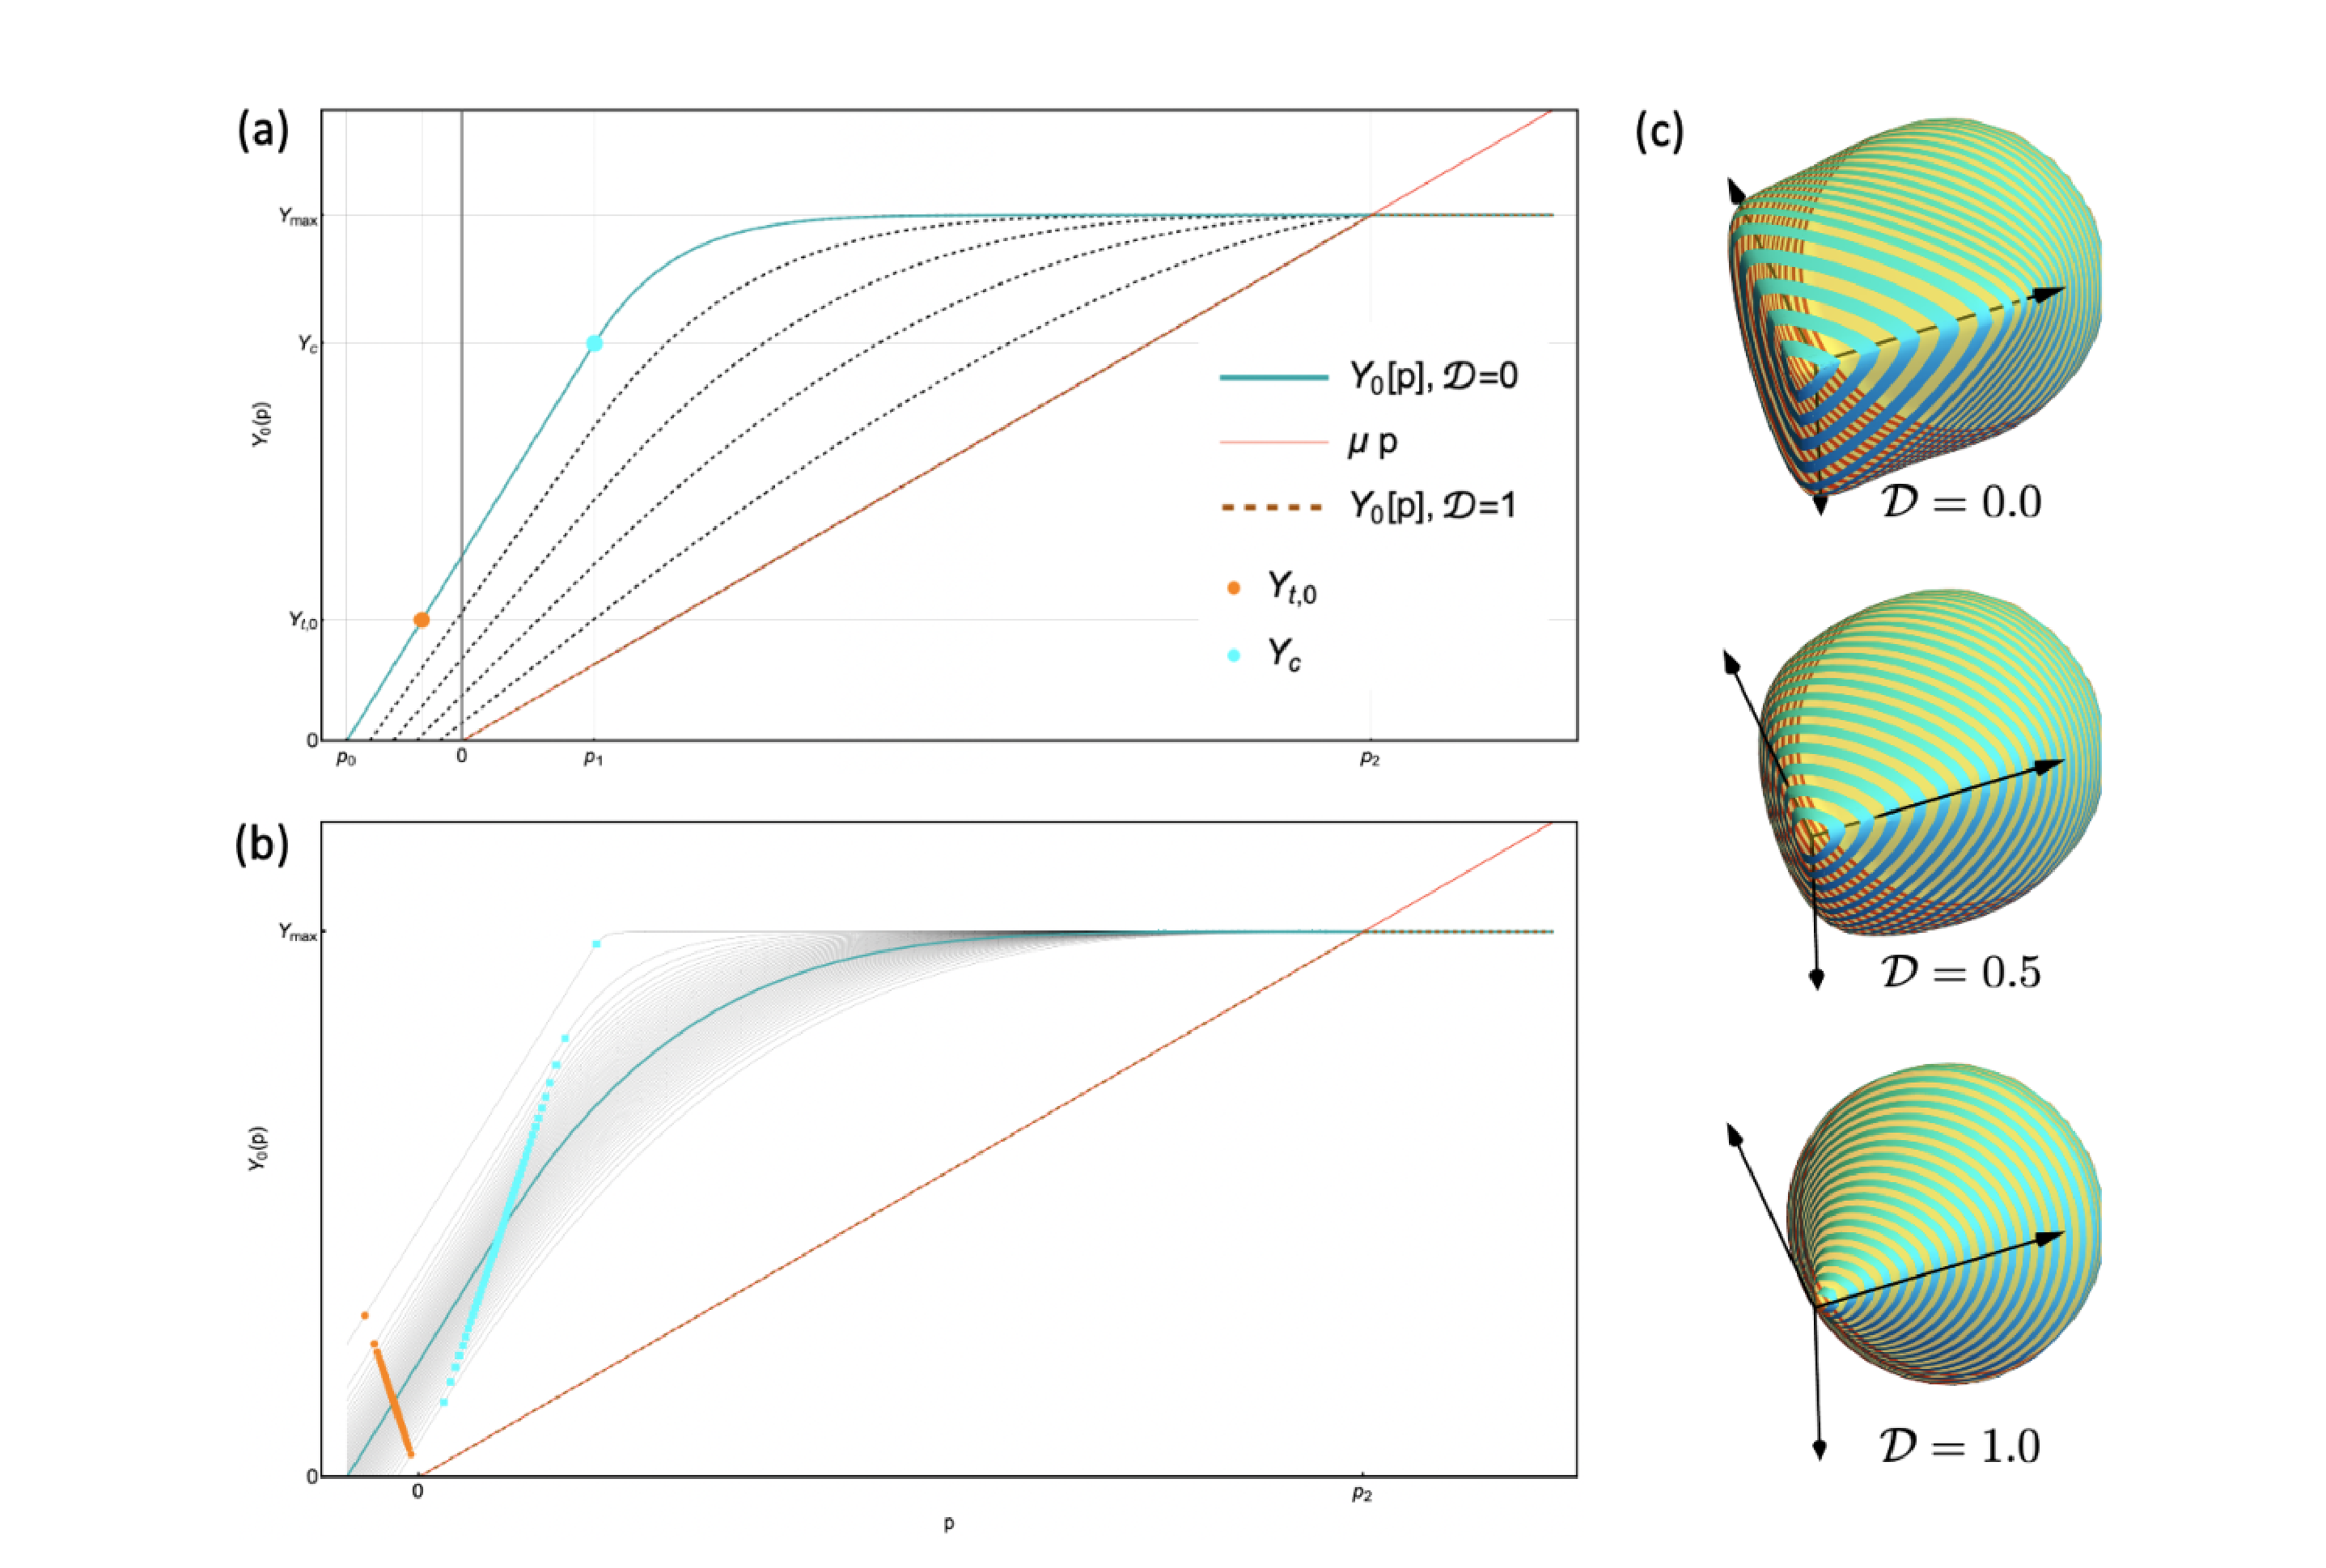
\includegraphics[width=0.92\linewidth]{figures/ceramic_damage_yield_surface_fig8_hi.pdf}
  \caption{Yield surface used by the isotropic ceramic damage model.  Panel (a) shows the pressure-dependent meridional strength without third-invariant dependence, evolving from intact to damaged states.  Panel (b) shows Weibull/strength-scale perturbations of the tensile and compressive strengths subject to the high-pressure cap.  Panel (c) shows the initial principal-stress-space surface for several damage values, illustrating the transition from low-pressure tensile failure toward high-pressure shear strength.  Adapted from Fig.~8 of Homel, Crook, and Appleton~\cite{homelCrookAppleton2026sizeeffects}.}
  \label{fig:ceramic-damage-yield-surface}
\end{figure}

\paragraph{Return mapping.}
The implementation uses a simple radial return in deviatoric stress.  After the pressure branch is selected, the trial deviatoric direction is retained and the returned shear magnitude is limited by the damaged strength,
\begin{equation}
  q^{n+1}=\min\left(q^{\mathrm{tr}},Y(p^{\mathrm{tr}},D,J_2,J_3)/\xi_{\mathrm{tip}}\right),
  \qquad
  \boldsymbol{\sigma}^{n+1}=-p^{n+1}\mathbf{I}+\frac{q^{n+1}}{q^{\mathrm{tr}}}\mathbf{s}^{\mathrm{tr}}.
  \label{eq:ceramic-radial-return}
\end{equation}
The elastic strain energy stored at the returned state is evaluated as
\begin{equation}
  W_e = \frac{(p^{n+1})^2}{2K_{\mathrm{eff}}}+\frac{(q^{n+1})^2}{6G},
  \label{eq:ceramic-elastic-energy}
\end{equation}
which is used by the energy-regularized damage path.  The stored \texttt{plasticStrain} is a diagnostic/history measure computed from the difference between the elastic strain increment implied by the stress change and the total strain increment; it should not be interpreted as a fully associative plastic-flow solution.

\paragraph{Damage regularization options.}
Two damage-progression paths are implemented.  The older time-to-failure path is selected when \texttt{enableEnergyFailureCriterion=0}.  If the trial state yields below the brittle-ductile transition pressure \(p_2\), damage increases according to
\begin{equation}
  D^{n+1}=\min\left(1,D^n+\frac{\Delta t}{t_f}\right),
  \qquad
  t_f=\frac{\ell_{\mathrm{ch}}}{c_f},
  \label{eq:ceramic-time-to-failure}
\end{equation}
where \(\ell_{\mathrm{ch}}=\texttt{lengthScale}\) and \(c_f=\texttt{crackSpeed}\).  This is computationally inexpensive and useful for simple damage growth studies, but the fracture energy is controlled only indirectly by \(c_f\), \(\ell_{\mathrm{ch}}\), and the stress history.

The energy-regularized path is selected when \texttt{enableEnergyFailureCriterion=1}.  In that branch the model tracks accumulated stress work \(W\) and compares the dissipated work \(W-W_e\) to the regularized fracture-energy density \(G_f/\ell_{\mathrm{ch}}\):
\begin{equation}
  D^{n+1}\approx
  \operatorname{clip}\left(\frac{W^{n+1}-W_e^{n+1}}{G_f/\ell_{\mathrm{ch}}},D^n,1\right).
  \label{eq:ceramic-energy-damage}
\end{equation}
If the strain energy at failure is small enough for a gradual softening process, the update performs a fixed-point iteration on \(D\).  If the strain energy at the failure stress already exceeds the target fracture dissipation for the current \(\ell_{\mathrm{ch}}\), the update instead uses a bisection solve for a partially relaxed damage state and sets \texttt{surfaceFlag=1} once the dissipated work reaches approximately \(G_f/\ell_{\mathrm{ch}}\).  That flag is what makes the option useful with DFG: the continuum law can release only the required amount of energy, while the kinematic enrichment creates a contact-capable fracture surface so the residual elastic energy drives opening or slip rather than being smeared into a continuum porosity field.  The regularization concept follows the Homel-Crook-Appleton kinematic-regularization discussion, in which damage, surface insertion, and the energy budget are decoupled when a cell is too large to resolve the fracture process zone~\cite{homelCrookAppleton2026sizeeffects}.

\paragraph{Strength scale and crack-tip scaling.}
The \texttt{strengthScale} field is applied directly to \(Y_t\) and \(Y_c\), so Weibull or spatial heterogeneity assigned by PFW affects both tensile and compressive branches while leaving \(Y_{\max}\) as the limiting ductile strength.  This is the model-specific interpretation of the shared strength-scale field described in Section~\ref{subsubsec:strength-scale-weibull}.  In DFG fracture calculations, \texttt{strengthScale} is commonly assigned by Voronoi/Weibull wrappers so that the initial critical flaws occupy clusters of particles rather than isolated particles.

When crack-tip scaling is enabled, the solver supplies \texttt{distanceToCrackTip} from the neighbor-list DFG crack-tip diagnostic.  The model computes a fracture-process-zone radius from the nominal intact strength,
\begin{equation}
  r_p = \frac{K_{Ic}^{2}}{2\pi Y_{\text{intact}}^{2}},
  \qquad
  \xi_{\mathrm{tip}} = \max\left(1,\sqrt{\frac{r}{r_p}}\right),
  \label{eq:ceramic-crack-tip-factor}
\end{equation}
and divides the effective strength by \(\xi_{\mathrm{tip}}\) when evaluating the yield condition and the return surface.  The stress that is stored and used in momentum balance is not multiplied by this factor; the factor modifies the damage/fracture criterion to represent under-resolved near-tip stresses.  This links the ceramic model to the shared crack-tip modifier in Section~\ref{subsubsec:crack-tip-stress-concentration}.  The uploaded Homel-Crook-Appleton manuscript describes the same idea: the crack-tip factor affects the propagation criterion, while the final output stress and stress work are computed with the unscaled stress~\cite{homelCrookAppleton2026sizeeffects}.

\paragraph{DFG use and porosity interpretation.}
The model can run without DFG, but its intended brittle-fracture workflow is \texttt{CeramicDamage}+DFG.  Without DFG, a fully damaged region remains a continuum carried by the single MPM velocity field and can smear damaged/intact kinematics.  With DFG, particles near a sufficiently sharp damage gradient can be split into two velocity fields, and the contact algorithm then supplies frictional slip and separation on the inserted fracture.  This is important for ceramics, concrete mesostructures, and brittle granular aggregates, where post-failure deformation is often controlled by relative motion of rough fracture faces or fragments.  The \texttt{porosity} field in \texttt{CeramicDamage} currently scales strength through Eq.~\eqref{eq:ceramic-strength-porosity-scale}; it should not be used as the primary representation of dilation caused by fracture slip.  If the problem requires an evolving continuum porosity, pore-pressure coupling, pore collapse, or compaction-induced void-ratio evolution, use or extend \texttt{Geomechanics} (Section~\ref{subsubsec:geomechanics-model}) rather than interpreting DFG fracture dilation as a scalar porosity increment.

\clearpage
\paragraph{Implementation pseudocode.}\mbox{}\par\smallskip
\begin{lstlisting}[caption={CeramicDamage update structure.},label={alg:ceramic-damage-update},basicstyle=\ttfamily\small]
read D, J, lengthScale, strengthScale, porosity, distanceToCrackTip
Yt = strengthScale * (1 - porosity) * tensileStrength
Yc = strengthScale * (1 - porosity) * compressiveStrength
cap Yc by maximumStrength and form Yt0 for optional third-invariant scaling
p_trial = -K_eff(D,J) * log(J)
q_trial, J2, J3, s_hat = deviatoric_invariants(trialStress)
Y_intact = strength(p_trial, D=0, xi=1, J2, J3)
if crack_tip_option and distanceToCrackTip > 0:
  rp = fractureToughness^2 / (2*pi*Y_intact^2)
  xi = max(1, sqrt(distanceToCrackTip / rp))
else:
  xi = 1
Y = strength(p_trial, D, xi, J2, J3)
if p_trial >= (1-D)*p0 and q_trial <= Y:
  accept trial stress
  if energy criterion: accumulatedWork += stress : strainIncrement
else:
  if energy criterion:
    iterate D so (accumulatedWork - elasticEnergy) ~= Gf/lengthScale
    if target dissipation reached: surfaceFlag = 1
  else:
    if p_trial < maximumStrength/frictionSlope:
      D = min(1, D + dt / (lengthScale/crackSpeed))
  radial_return_to_strength_surface(D, xi)
update plasticStrain diagnostic and store stress, D, work, surfaceFlag
\end{lstlisting}

\subsubsection{\texttt{Chiumenti}}
\label{subsubsec:chiumenti-model}
\index{constitutiveModels!Chiumenti}
\index{Rankine damage}

\texttt{Chiumenti} is a scalar tensile-damage model built on the \texttt{HyperelasticMMS} trial stress.  It follows the local continuum damage / crack-band style of Rankine tensile softening used in the work of Cervera and Chiumenti~\cite{cervera2006chiumenti}.  In GEOS-MPM, it provides a compact hyperelastic-damage option for cases that require tensile degradation with a characteristic length and fracture-energy parameter, but not the full ceramic or geomechanics response.

The model computes a hyperelastic trial stress, obtains principal stresses \(\sigma_i\), and defines a strength
\begin{equation}
  Y_f = s_p Y_{f0},
\end{equation}
where \(s_p\) is the particle \texttt{strengthScale}.  With Young's modulus \(E\), critical length \(\ell_c\), and energy-release parameter \(G_f\), the implementation uses a brittleness factor
\begin{equation}
  b = \frac{Y_f^2}{2 E G_f},
  \qquad
  b_c = \frac{b\ell_c}{1-b\ell_c}.
  \label{eq:chiumenti-brittleness}
\end{equation}
When the maximum tensile principal stress \(\sigma_{\max}\) exceeds \(Y_f\), the damage candidate is
\begin{equation}
  D_{\mathrm{new}}
  = (1+b_c)\left(1-\frac{Y_f}{\sigma_{\max}}\right),
  \qquad
  D^{n+1}=\max\left(D^n,\min(1,\max(0,D_{\mathrm{new}}))\right).
  \label{eq:chiumenti-damage}
\end{equation}
Positive principal stresses are then degraded by \(1-D\), while compressive principal stresses are left unchanged.

\begin{lstlisting}[caption={Chiumenti tensile-damage update.},label={alg:chiumenti-update},basicstyle=\ttfamily\small]
stress_trial = HyperelasticMMS(F)
if inelasticity disabled: return stress_trial
Yf = failureStrength * strengthScale
principalStress, eigenvectors = eig(stress_trial)
sigmaMax = max(max(principalStress), 0)
if sigmaMax > Yf:
  b = Yf^2 / (2 * E * energyReleaseRate)
  bc = b * criticalLength / (1 - b * criticalLength)
  damage = max(oldDamage, clamp((1 + bc) * (1 - Yf/sigmaMax), 0, 1))
for each principal stress i:
  if principalStress[i] > 0: principalStress[i] *= (1 - damage)
stress = recompose(principalStress, eigenvectors)
\end{lstlisting}
\subsubsection{\texttt{Graphite}}
\label{subsubsec:graphite-model}
\index{constitutiveModels!Graphite}
\index{Graphite model}
\index{MaterialDirection!Graphite}
\index{transverse isotropy!Graphite}
\index{graphite!weak planes}
\index{graphite!basal planes}
\index{graphite!point-slope strength}

\texttt{Graphite} is an anisotropic damage/plasticity model for graphite-like layered solids.  The model assumes that the material has a preferred graphitic or basal-plane normal, stored as the first row of the particle \texttt{MaterialDirection} tensor.  The weak planes themselves are normal to this vector.  The constitutive update therefore treats the particle material direction as a plane normal, not as an ordinary fiber tangent.  This distinction matters in large deformation: ordinary line directions are pushed forward with \(\mathbf F\), while plane normals are pushed forward with the deformation-gradient cofactor \(\mathbf F^{c}=J\mathbf F^{-T}\).  The MPM kinematic update uses this cofactor path for non-fiber material directions, normalizes the transported rows, and then passes the updated material basis to the constitutive model.  This is the appropriate graphitic update because the orientation of a basal plane is controlled by the transformed plane normal rather than by the stretch of an in-plane material line; see also the material-direction assignment discussion in Section~\ref{subsec:pfw-material-directions}.  The need to distinguish material rotations, basis transformations, and evolving anisotropy is the same tensor-transformation issue emphasized by Brannon's rotation and frame-change treatment~\cite{brannon2017rotation}.

\begin{figure}[htbp]
  \centering
  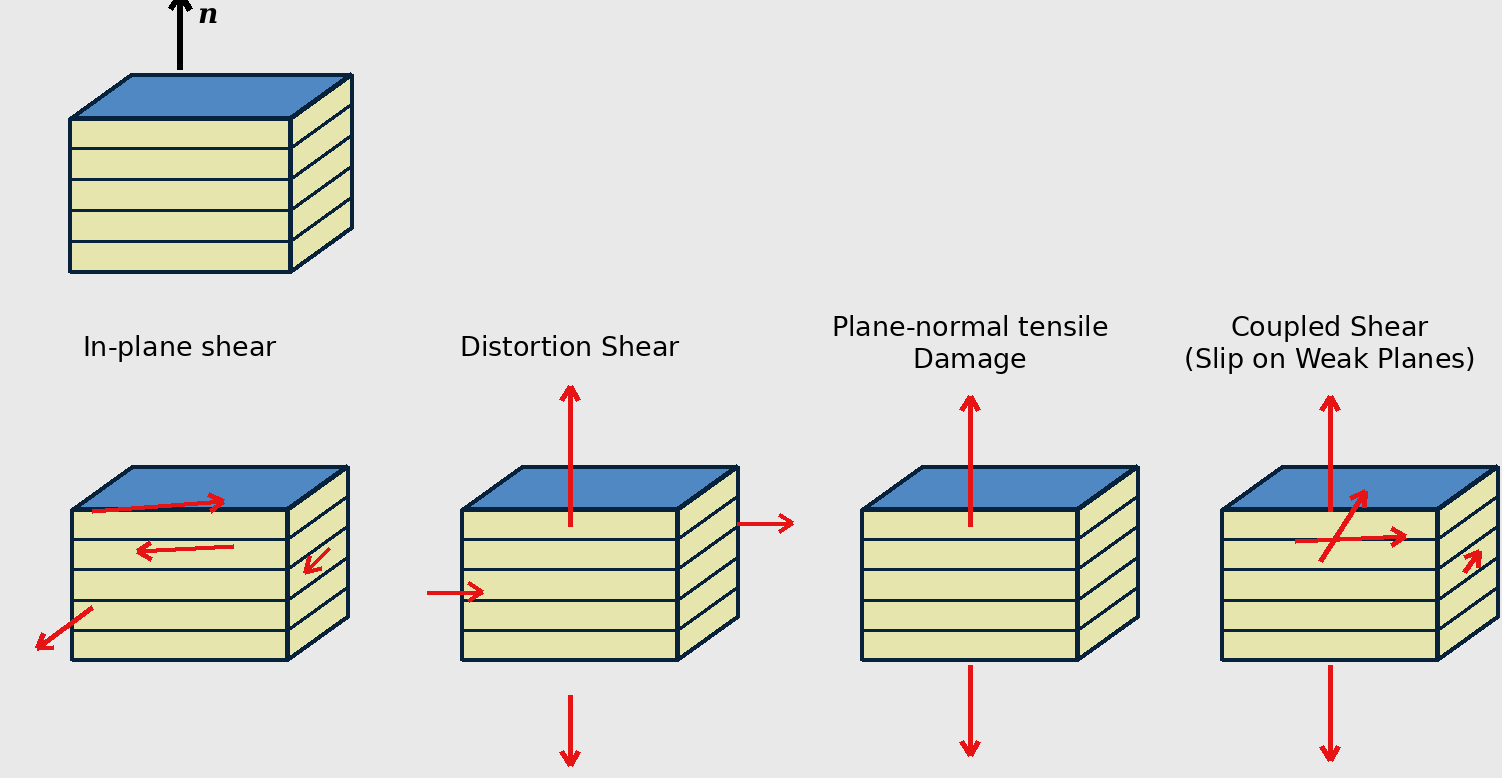
\includegraphics[width=0.96\linewidth]{figures/graphite_deformation_modes.png}
  \caption{Graphite weak-plane deformation modes.  The supplied diagram illustrates the basal-plane normal, in-plane shear, distortion shear, plane-normal tensile damage, and coupled shear/slip on weak planes.  The assigned material direction \(\mathbf a\) is the normal to the weak graphitic planes; in-plane, distortion, plane-normal, and coupled weak-plane stress modes are limited by separate pressure-dependent strength functions.}
  \label{fig:graphite-deformation-modes}
\end{figure}

\paragraph{Kinematics and material basis.}
Let \(\mathbf a\) be the current unit normal to the graphitic planes and let
\begin{equation}
  \mathbf M = \mathbf a\otimes\mathbf a,
  \qquad
  \mathbf P = \mathbf I - \mathbf M,
  \label{eq:graphite-projectors}
\end{equation}
where \(\mathbf P\) projects onto the basal plane.  In the current implementation the full particle material basis is stored row-wise, but the constitutive update uses only the first row as \(\mathbf a\).  The solver first transports the reference basis by
\begin{equation}
  \mathbf A^{\mathrm{trial}} =
  \begin{cases}
    \mathbf F\mathbf A_0^T, & \hbox{fiber-like material directions},\\
    \mathbf F^{c}\mathbf A_0^T, & \hbox{graphitic plane normals and other non-fiber directions},
  \end{cases}
  \qquad
  \mathbf F^{c}=J\mathbf F^{-T},
  \label{eq:graphite-material-direction-update}
\end{equation}
then transposes and normalizes the rows to recover the particle \texttt{MaterialDirection}.  Inside the constitutive update, the beginning-of-step rotation is removed before evaluating the transversely isotropic elastic and inelastic laws, so the mode decomposition is performed in a corotational material frame.  This path is consistent with the general rule that anisotropic constitutive models must evolve their material directions under superposed rigid motion and finite distortion, rather than treating a fixed laboratory axis as a material property~\cite{brannon2017rotation}.

\paragraph{Elastic trial stress.}
The reviewed code path is a finite-deformation MPM update followed by a corotational transversely isotropic elastic predictor.  The implementation is compatible with the hyperelastic transversely isotropic interpretation of the model, but the update evaluated here is algorithmically a pressure-dependent rate-form trial stress expressed in the evolving material frame.  The pressure-dependent moduli are computed from the beginning-of-step pressure \(p^n=-\operatorname{tr}\boldsymbol{\sigma}^n/3\) and the beginning-of-step plane-normal stress \(\sigma_n^n=\mathbf a\cdot\boldsymbol{\sigma}^n\mathbf a\).  Define the non-negative arguments
\begin{equation}
  \xi_z = \max\left(0,\frac{p^n-\sigma_n^n}{2}\right),
  \qquad
  \xi_p = \max(0,p^n),
  \label{eq:graphite-elastic-pressure-arguments}
\end{equation}
and the saturating pressure function
\begin{equation}
  f(\xi;P)=\frac{\xi}{1+\xi/P}.
  \label{eq:graphite-saturating-pressure-function}
\end{equation}
Then
\begin{align}
  E_z &= \max\left(10^{-3}E_z^0,
       E_z^0 + E_z' f(\xi_z;P_z)\right),\\
  E_p &= \max\left(10^{-3}E_p^0,
       E_p^0 + E_p' f(\xi_p;P_p)\right),\\
  G_{zp} &= \max\left(10^{-3}G_{zp}^0,
       G_{zp}^0 + G_{zp}' f(\xi_p;P_g)\right),\\
  \nu_{zp} &= \min(0.4999,\nu_{zp}^0),
  \qquad
  \nu_p = \min(0.4999,\nu_p^0).
  \label{eq:graphite-pressure-dependent-moduli}
\end{align}
Here \(z\) denotes the preferred-axis direction and \(p\) denotes the transverse plane.  The optional pressure scales \(P_z\), \(P_p\), and \(P_g\) are supplied by \texttt{defaultYoungModulusAxialPressureScale}, \texttt{defaultYoungModulusTransversePressureScale}, and \texttt{defaultShearModulusAxialTransversePressureScale}.  When a pressure scale is omitted, its default is effectively infinite and \(f(\xi;P)\to\xi\), recovering the linear pressure dependence.  Finite positive scales give monotone pressure stiffening with decreasing tangent modulus increment at high pressure.  The implementation also locally limits the pressure-dependent TI moduli if needed so the stiffness remains positive definite at the current pressure state.  The implementation also forms effective isotropic moduli for wave-speed and stress-control purposes,
\begin{equation}
  K_{\mathrm{eff}} =
  -\frac{E_pE_z}{2E_z(\nu_p+\nu_{zp}-1)+E_p(2\nu_{zp}-1)},
  \qquad
  G_{\mathrm{eff}} = 0.6K_{\mathrm{eff}}.
  \label{eq:graphite-effective-moduli}
\end{equation}

The elastic stiffness is written using the five transversely isotropic fourth-order basis tensors associated with the symmetry axis \(\mathbf a\).  Brannon gives the corresponding TI basis and discusses the physical meaning of these components as axial response, in-plane isotropic response, Poisson coupling, in-plane shear, and shear involving the symmetry axis~\cite{brannon2017rotation}.  In component form, with \(a_i\) denoting the components of \(\mathbf a\),
\begin{align}
  B^{(1)}_{ijpw} &= a_i a_j a_p a_w,\\
  B^{(2)}_{ijpw} &= \delta_{ij}\delta_{pw}
      -a_i a_j\delta_{pw}-\delta_{ij}a_p a_w+a_i a_j a_p a_w,\\
  B^{(3)}_{ijpw} &= a_i a_j\delta_{pw}+\delta_{ij}a_p a_w
      -2a_i a_j a_p a_w,\\
  B^{(4)}_{ijpw} &= \frac{1}{2}\left(\delta_{ip}\delta_{jw}+\delta_{iw}\delta_{jp}\right)
      -\frac{1}{2}\left(\delta_{iw}a_j a_p+a_i\delta_{jp}a_w+a_i\delta_{jw}a_p+\delta_{ip}a_j a_w\right)
      +a_i a_j a_p a_w,\\
  B^{(5)}_{ijpw} &= \frac{1}{2}\left(\delta_{ip}a_j a_w+\delta_{iw}a_j a_p+a_i\delta_{jw}a_p+a_i\delta_{jp}a_w\right)
      -2a_i a_j a_p a_w.
  \label{eq:graphite-ti-basis}
\end{align}
The stiffness used by the trial update is
\begin{equation}
  \mathbb C_{\mathrm{TI}} = h_1\mathbb B^{(1)}+h_2\mathbb B^{(2)}+h_3\mathbb B^{(3)}+h_4\mathbb B^{(4)}+h_5\mathbb B^{(5)},
  \label{eq:graphite-ti-stiffness}
\end{equation}
with
\begin{align}
  h_1 &= \frac{E_z^2(\nu_p-1)}{E_z(\nu_p-1)+2E_p\nu_{zp}^2},
  &
  h_2 &= -\frac{E_p(E_z\nu_p+E_p\nu_{zp}^2)}{(1+\nu_p)\left[E_z(\nu_p-1)+2E_p\nu_{zp}^2\right]},\\
  h_3 &= \frac{E_pE_z\nu_{zp}}{E_z-E_z\nu_p-2E_p\nu_{zp}^2},
  &
  h_4 &= \frac{E_p}{1+\nu_p},
  &
  h_5 &= 2G_{zp}.
  \label{eq:graphite-h-coefficients}
\end{align}
The trial stress increment is
\begin{equation}
  \Delta\boldsymbol{\sigma}^{\mathrm{tr}}
  = \mathbb C_{\mathrm{TI}}:
  \left(\mathbf D - \boldsymbol{\alpha}\dot T\right)\Delta t,
  \qquad
  \boldsymbol{\alpha} = (\alpha_L-\alpha_T)\mathbf a\otimes\mathbf a+\alpha_T\mathbf I,
  \label{eq:graphite-trial-stress}
\end{equation}
where \(\dot T=\texttt{temperatureRate}\).  Thus thermal expansion is anisotropic: \(\alpha_L\) is applied along the symmetry-axis normal and \(\alpha_T\) in the basal plane.  In current GEOS-MPM workflows, \texttt{temperature} and \texttt{temperatureRate} are generally prescribed by global solver events that define a transient thermal response; the graphite update consumes these fields to represent thermal expansion and temperature-dependent properties.  A future coupled heat-transfer solver could instead define local particle temperature and temperature-rate fields.

\paragraph{Mode decomposition of stress.}
After the trial stress is computed, the model decomposes it into four symmetric tensor parts.  In the notation of Eq.~\eqref{eq:graphite-ti-basis},
\begin{align}
  \boldsymbol{\sigma}_1 &= \mathbb B^{(1)}:\boldsymbol{\sigma},
  &\hbox{plane-normal/axial part},\\
  \boldsymbol{\sigma}_2 &= \mathbb B^{(2)}:\boldsymbol{\sigma},
  &\hbox{in-plane isotropic part before the factor }1/2,\\
  \boldsymbol{\sigma}_4 &= \mathbb B^{(4)}:\boldsymbol{\sigma},
  &\hbox{in-plane total part},\\
  \boldsymbol{\sigma}_5 &= \mathbb B^{(5)}:\boldsymbol{\sigma},
  &\hbox{coupled weak-plane shear part}.
  \label{eq:graphite-stress-parts}
\end{align}
The in-plane isotropic contribution used for reconstruction is \(\boldsymbol{\sigma}_{\mathrm{ip}}^{\mathrm{iso}}=\boldsymbol{\sigma}_2/2\), while the in-plane deviator is
\begin{equation}
  \boldsymbol{\sigma}_{\mathrm{ip}}^{\mathrm{dev}} = \boldsymbol{\sigma}_4 - \frac{1}{2}\boldsymbol{\sigma}_2 .
  \label{eq:graphite-inplane-dev}
\end{equation}
The distortion stress is the combination of the plane-normal and in-plane-isotropic parts,
\begin{equation}
  \boldsymbol{\sigma}_{\mathrm{dist}} = \boldsymbol{\sigma}_1 + \frac{1}{2}\boldsymbol{\sigma}_2,
  \qquad
  \boldsymbol{\sigma}_{\mathrm{dist}}^{\mathrm{dev}} =
  \operatorname{dev}\boldsymbol{\sigma}_{\mathrm{dist}}.
  \label{eq:graphite-distortion-stress}
\end{equation}
The signed distortion invariant is
\begin{equation}
  I_d = \sigma_{aa} - \frac{\sigma_{bb}+\sigma_{cc}}{2},
  \qquad
  I_d^+ = \langle I_d\rangle_+,
  \qquad
  I_d^- = \langle -I_d\rangle_+,
  \label{eq:graphite-signed-distortion}
\end{equation}
where \(\mathbf a\) is the basal-plane normal and \(\mathbf b,\mathbf c\) span the basal plane.  The scalar \(|I_d|\) is equal to \(\sqrt{3/2}\|\boldsymbol{\sigma}_{\mathrm{dist}}^{\mathrm{dev}}\|\), but the split form allows the model to assign different strengths to basal-normal relative compression and basal-normal relative extension/opening-like distortion.  The remaining mode invariants use Mandel-consistent norms,
\begin{equation}
  q_{\mathrm{ip}} = \sqrt{\frac{3}{2}}\,\|\boldsymbol{\sigma}_{\mathrm{ip}}^{\mathrm{dev}}\|,
  \qquad
  q_{\mathrm{c}} = \sqrt{\frac{3}{2}}\,\|\boldsymbol{\sigma}_5\|.
  \label{eq:graphite-mode-invariants}
\end{equation}
These are the internal stress measures corresponding to signed normal distortion, in-plane shear, and coupled shear on the graphitic weak planes in Fig.~\ref{fig:graphite-deformation-modes}.  Plane-normal tensile opening is handled separately by comparing \(\sigma_n=\mathbf a\cdot\boldsymbol{\sigma}\mathbf a\) with \texttt{failureStrength}.

\paragraph{Pressure-dependent point-slope strengths.}
Each active strength branch \(m\in\{d-,d+,\mathrm{ip},\mathrm{c}\}\) has a pressure-dependent strength curve controlled by \texttt{*ResponseX2}, \texttt{*ResponseY1}, \texttt{*ResponseY2}, and \texttt{*ResponseM1}.  The existing \texttt{distortionShearResponse*} inputs define the \(I_d^-\) branch.  The optional \texttt{positiveDistortionShearResponse*} inputs define the \(I_d^+\) branch and default to the corresponding \texttt{distortionShearResponse*} values when omitted, so old input files recover the previous unsigned distortion response.  With \(x_1=0\), \(x_2>0\), \(Y_1\ge 0\), \(Y_2>Y_1\), and low-pressure tangent slope \(M_1\), the code uses a point-slope form
\begin{equation}
Y_m(p)=
\begin{cases}
  \max\left(0, Y_1-(x_1-p)M_1\right), & p<x_1,\\[0.4em]
  Y_2+(Y_1-Y_2)\left(\dfrac{p-x_2}{x_1-x_2}\right)^{M_1(x_1-x_2)/(Y_1-Y_2)}, & x_1\le p < x_2,\\[0.8em]
  Y_2, & p\ge x_2.
\end{cases}
\label{eq:graphite-point-slope-strength}
\end{equation}
This curve passes through \((x_1,Y_1)\) with derivative \(M_1\), passes through \((x_2,Y_2)\), and is tangent to the high-pressure branch, which is a zero-slope plateau in the present form.  The elastic domain is convex only if the low-pressure slope is steeper than the secant slope, so the intended parameter regime is
\begin{equation}
  M_1 > \frac{Y_2-Y_1}{x_2-x_1}.
  \label{eq:graphite-point-slope-convexity}
\end{equation}
After damage and hardening modifications the implementation enforces this condition by increasing \(M_1\) when needed, with a small numerical margin in production inputs preferred over exact equality.

\begin{figure}[htbp]
  \centering
  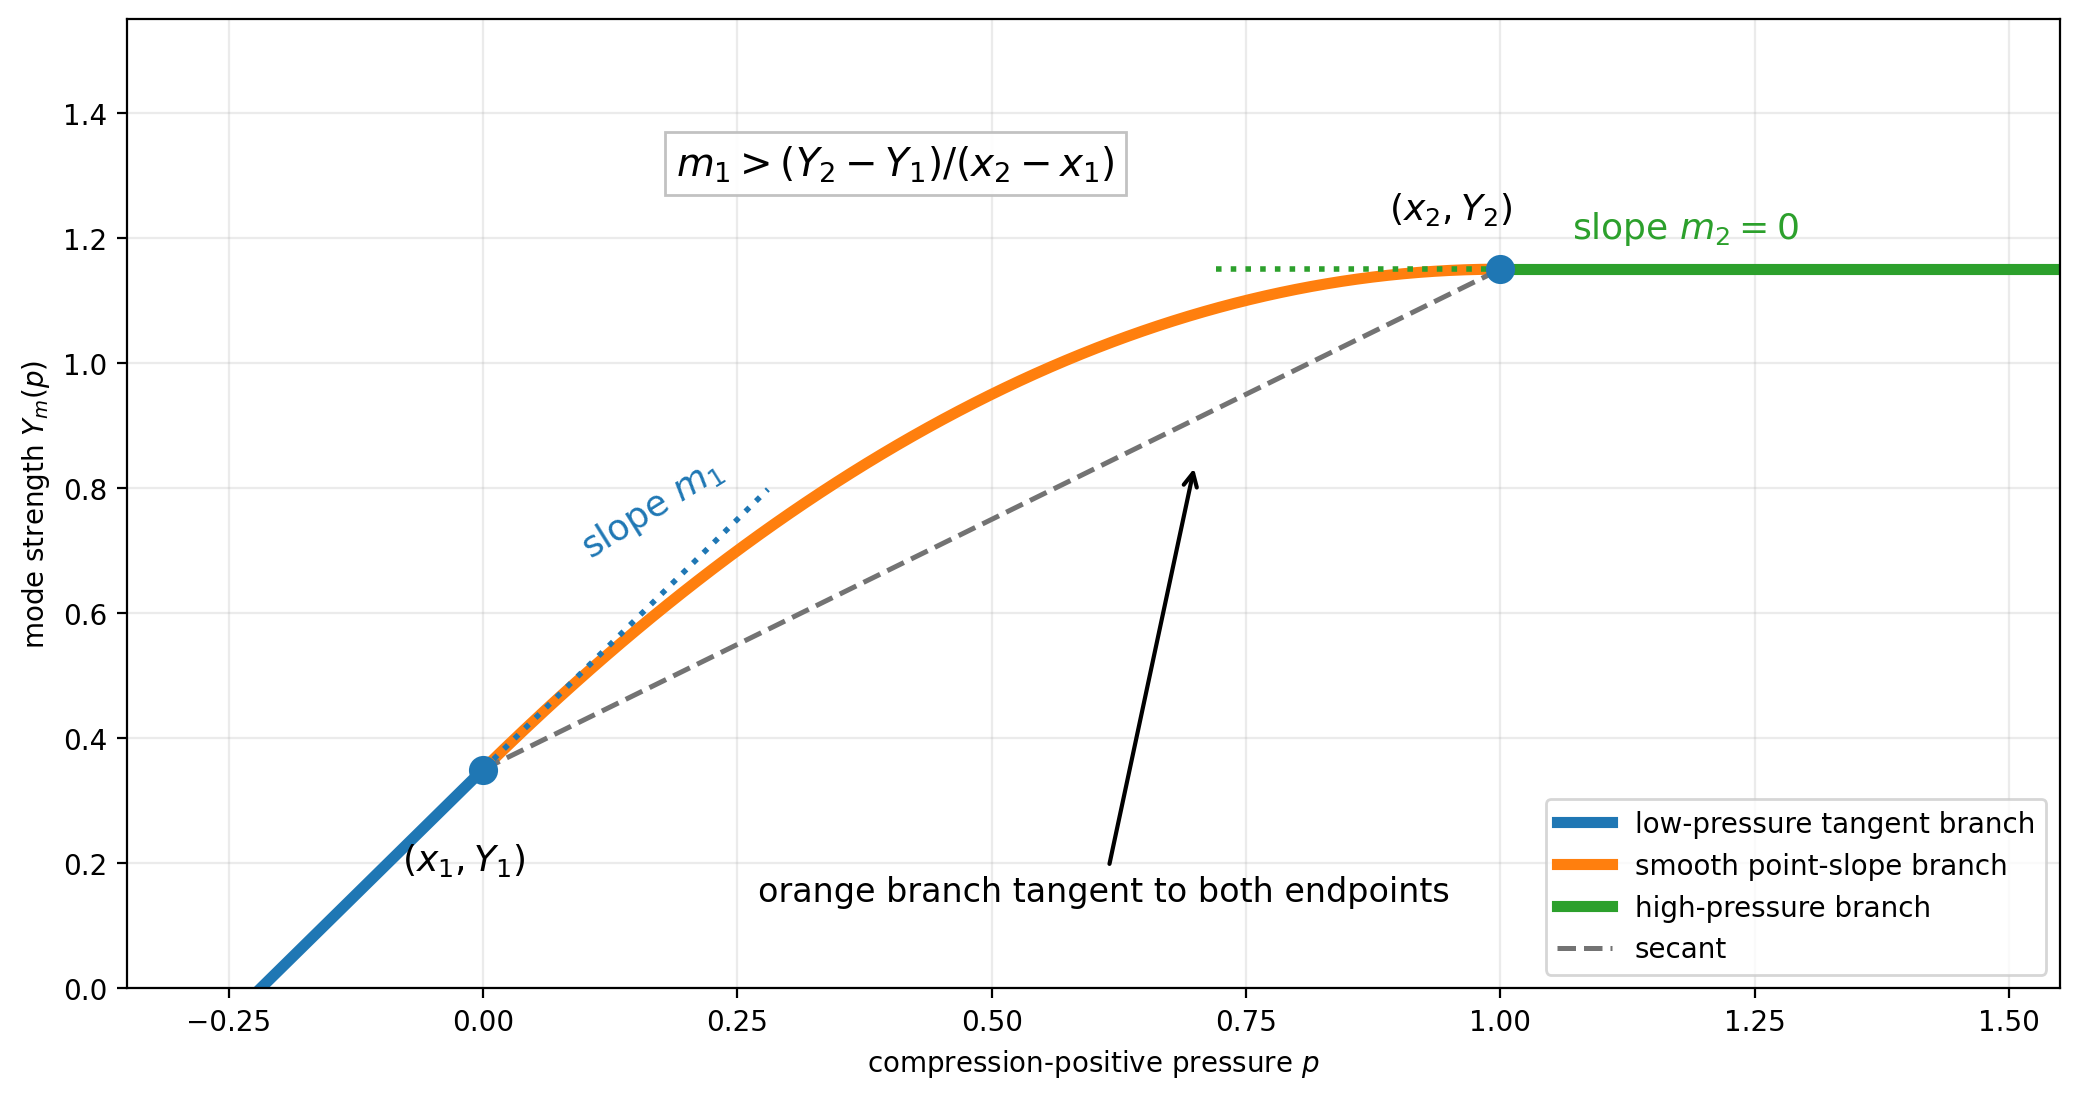
\includegraphics[width=0.78\linewidth]{figures/graphite_point_slope_strength.png}
  \caption{Pressure-dependent point-slope strength form used for each active graphite strength branch, including the signed distortion branches, in-plane shear, and coupled weak-plane shear.  The orange transition is constructed to be tangent to the low-pressure branch at \((x_1,Y_1)\) and tangent to the high-pressure plateau at \((x_2,Y_2)\); convexity requires \(M_1>(Y_2-Y_1)/(x_2-x_1)\).}
  \label{fig:graphite-point-slope-strength}
\end{figure}

Damage, strength scaling, and hardening modify the raw input strengths before Eq.~\eqref{eq:graphite-point-slope-strength} is evaluated.  Let \(s_p=\texttt{strengthScale}\), \(D_m\in[0,1]\) be the internal mode damage used for a branch, \(\chi=\texttt{relaxation}\in[0,1]\) be the accumulated plastic-strain hardening coordinate, and
\begin{equation}
  S(\chi)=3\chi^2-2\chi^3,
  \qquad
  H_m(\chi)=1+(C_m-1)S(\chi).
  \label{eq:graphite-hardening-multiplier}
\end{equation}
Here \(C_m\) is one of \texttt{distortionStrainHardeningC0}, \texttt{inPlaneStrainHardeningC0}, or \texttt{coupledStrainHardeningC0}; both signed distortion branches use the distortion hardening multiplier.  The intact low-pressure ordinate and tangent slope are scaled by \(s_pH_m\), but the high-pressure plateau is not strength-scale multiplied:
\begin{equation}
  Y_{1,\mathrm{intact}} = \min\left(s_pH_mY_1^0,(1-\epsilon)Y_2^0\right),
  \qquad
  Y_{2,\mathrm{intact}} = Y_2^0.
  \label{eq:graphite-strengthscale-damage}
\end{equation}
The intact slope is raised as needed to satisfy the convexity condition in Eq.~\eqref{eq:graphite-point-slope-convexity}.  The fully comminuted powder branch has zero cohesion, uses \texttt{damagedMaterialFrictionalSlope} subject to the same slope limits, and retains the same unscaled branch-specific \(Y_2^0\) plateau.  The active strength is a smooth blend of the intact and powder branches using the internal damage variable for that mode.  This makes \texttt{strengthScale} a flaw-controlled low-pressure multiplier while preserving a common pressure-dominated high-confinement strength for intact and comminuted material.  Fracture energies may be scaled separately through \(G_f^{\mathrm{eff}}=G_f\,s_p^{\eta_G}\), where \(\eta_G=\texttt{fractureEnergyStrengthScaleExponent}\).

\paragraph{Mode return and reconstruction.}
The inelastic correction uses a single quadratic TI strength index,
\begin{equation}
  R^2 =
  \left(\frac{I_d^+}{Y_{d+}(p)}\right)^2+
  \left(\frac{I_d^-}{Y_{d-}(p)}\right)^2+
  \left(\frac{q_{\mathrm{ip}}}{Y_{\mathrm{ip}}(p)}\right)^2+
  \left(\frac{q_{\mathrm{c}}}{Y_{\mathrm{c}}(p)}\right)^2 .
  \label{eq:graphite-quadratic-ti-yield}
\end{equation}
When \(R>1\), the deviatoric distortion, in-plane, and coupled weak-plane stress parts are scaled by \(1/R\).  This is a radial projection onto a coupled anisotropic strength index rather than a full closest-point plasticity return.  After the correction, the stress is reconstructed as
\begin{equation}
  \boldsymbol{\sigma}^{n+1} =
  \boldsymbol{\sigma}_{\mathrm{dist}}^{\mathrm{iso}}
  + \boldsymbol{\sigma}_{\mathrm{dist}}^{\mathrm{dev,capped}}
  + \boldsymbol{\sigma}_{\mathrm{ip}}^{\mathrm{dev,capped}}
  + \boldsymbol{\sigma}_{5}^{\mathrm{capped}}.
  \label{eq:graphite-stress-reconstruction}
\end{equation}
For fully damaged particles, the implementation also removes tensile plane-normal stress and spherical tensile distortion stress, so the damaged material can continue to carry compressive/frictional response but cannot support cohesive opening strength.

\paragraph{Plastic strain, hardening, and damage evolution.}
When at least one mode cap is active, the model computes a plastic strain increment by subtracting the elastic strain increment implied by the TI compliance from the total symmetric velocity-gradient increment.  The TI compliance uses coefficients
\begin{equation}
  s_1=\frac{1}{E_z},\qquad
  s_2=-\frac{\nu_p}{E_p},
  \qquad
  s_3=-\frac{\nu_{zp}}{E_z},
  \qquad
  s_4=\frac{1+\nu_p}{E_p},
  \qquad
  s_5=\frac{1}{2G_{zp}}.
  \label{eq:graphite-compliance-coefficients}
\end{equation}
The relaxation/hardening coordinate is then advanced approximately as
\begin{equation}
  \chi^{n+1}=\min\left(1,\chi^n+\frac{\|\Delta\boldsymbol{\epsilon}^p\|}{\epsilon^p_{\max}}\right),
  \label{eq:graphite-relaxation-update}
\end{equation}
where \(\epsilon^p_{\max}=\texttt{maximumPlasticStrain}\).  This history variable is the argument in Eq.~\eqref{eq:graphite-hardening-multiplier}.

Damage can evolve through several mechanisms.  First, when \texttt{maximumPrincipalStressDamage=1}, the model evaluates the largest principal stress and advances damage if
\begin{equation}
  C_{\mathrm{tip}}\,\sigma_{\max} > s_p\,\sigma_f,
  \label{eq:graphite-maxprincipal-damage}
\end{equation}
where \(\sigma_f=\texttt{failureStrength}\) and \(C_{\mathrm{tip}}=\texttt{crackTipStressConcentration}\).  The crack-tip multiplier is produced by the shared crack-tip modifier described in Section~\ref{subsubsec:crack-tip-stress-concentration}.  Second, if \texttt{crackSpeed} is finite and an inelastic correction has occurred, damage advances over the time-to-failure scale
\begin{equation}
  \Delta D = \frac{\Delta t}{\ell/c_f},
  \qquad
  \ell=\texttt{lengthScale},
  \quad c_f=\texttt{crackSpeed}.
  \label{eq:graphite-crackspeed-damage}
\end{equation}
Third, the model accumulates basal-plane plastic work and non-basal plastic work.  The basal work combines Mode-I basal-plane plastic opening work and basal-plane shear work; the total work path excludes the basal plane-normal and basal shear parts.  These work measures are regularized by fracture energy per unit characteristic length,
\begin{equation}
  D \leftarrow \max\left(D,
     \left[\min\left(1,\frac{W_b}{G_b/\ell}\right)\right]^{n_D},
     \left[\min\left(1,\frac{W_t}{G_t/\ell}\right)\right]^{n_D}
  \right),
  \label{eq:graphite-work-damage}
\end{equation}
where \(G_b=\texttt{basalPlaneFractureEnergyReleaseRate}\), \(G_t=\texttt{totalFractureEnergyReleaseRate}\), and \(n_D=\texttt{damageEvolutionExponent}\).  The effective fracture energy uses \(G_f^{\mathrm{eff}}=G_f s_p^{\eta_G}\), where \(\eta_G=\texttt{fractureEnergyStrengthScaleExponent}\).  If the exponent is omitted, the legacy \texttt{scaleFractureEnergyReleaseRate} flag initializes it to either zero or one.  Equation~\eqref{eq:graphite-work-damage} makes damage remain near zero until the accumulated work approaches the specified regularized fracture-work threshold, then ramps it toward one.

\paragraph{Thermal effects.}
Thermal effects in the current model enter through anisotropic thermal expansion in Eq.~\eqref{eq:graphite-trial-stress} and through any temperature-dependent parameter paths exposed by the material model.  In the current solver workflow, \texttt{temperature} and \texttt{temperatureRate} are normally imposed by global events, such as a \texttt{TemperatureProfile} or \texttt{TemperatureRamp}, to represent a prescribed transient thermal response.  The graphite constitutive update consumes \texttt{temperatureRate} to subtract \(\boldsymbol{\alpha}\dot T\) from the mechanical rate of deformation.  Local temperature fields could instead be supplied in the future by a coupled heat-transfer solver, because temperature is already a particle field shared by PFW initialization, events, output, and constitutive models as described in Section~\ref{subsubsec:constitutive-temperature}.

\paragraph{Update algorithm.}
\begin{lstlisting}[caption={Graphite constitutive update structure.},label={alg:graphite-update},basicstyle=\ttfamily\small]
read old stress, velocity gradient, F, materialDirection, damage, temperatureRate
transport/normalize material direction; use first row as basal-plane normal a
unrotate L and a into the corotational material frame
compute pressure p, plane-normal stress sigma_n, and saturating pressure-dependent TI moduli
construct TI stiffness from Brannon basis tensors B1...B5
stress_trial = oldStress + C_TI : (D - alpha * temperatureRate) * dt
if inelasticity is disabled: accept stress_trial

decompose stress_trial into sigma1, sigma2, sigma4, sigma5
compute signed distortion Id+/Id-, in-plane, and coupled shear invariants
compute branch strengths Y_d-, Y_d+, Y_ip, Y_c from point-slope curves
apply strengthScale to low-pressure intact branch only; keep Y2 unscaled
blend intact strengths toward pressure-dependent powder residual using internal damage
if R^2 = sum((mode stress)/(mode strength))^2 > 1: scale deviatoric TI modes by 1/R
reconstruct stress from corrected distortion, in-plane, and coupled parts
as damage grows: remove tensile plane-normal and spherical tensile strength

if any mode yielded:
  compute plastic strain increment from total strain increment minus TI elastic increment
  update relaxation/hardening coordinate
  update max-principal, crack-speed, basal-work, and total-work damage paths
store stress, damage, relaxation, plastic strain, plastic work, and diagnostics
\end{lstlisting}

\paragraph{Capabilities and limitations.}
The model is useful when the important physics are anisotropic graphitic weak planes, pressure-dependent shear strength, basal-plane slip/opening, thermal expansion anisotropy, and coupling to DFG fracture/contact.  It is not a general porous geomaterial model: continuum porosity, pore collapse, pressure-solution creep, and pore-pressure coupling should be handled by the \texttt{Geomechanics} family or by a future coupled model.  It is also not a fully coupled anisotropic plasticity return algorithm with a documented associated flow rule; the correction is a radial projection to a coupled TI strength index.  The strict stored-energy hyperelastic interpretation is likewise limited, because the reviewed code computes a corotational rate-form trial stress.  Finally, the constitutive update uses only the first material-direction row as the basal-plane normal, so users should initialize unused material-basis rows sensibly for robust kinematic transport and output, even though they do not directly alter the graphite strength calculation.

\begingroup
\footnotesize
\begin{longtable}{>{\raggedright\arraybackslash}p{0.44\linewidth}>{\raggedright\arraybackslash}p{0.49\linewidth}}
\caption{Main \texttt{Graphite} input groups.  See the generated schema appendix for exact defaults and registration status.\label{tab:graphite-parameters}}\\
\toprule
\textbf{Input group} & \textbf{Purpose}\\
\midrule
\endfirsthead
\toprule
\textbf{Input group} & \textbf{Purpose}\\
\midrule
\endhead
\texttt{defaultYoungModulusAxial}\newline \texttt{defaultYoungModulusTransverse}\newline \texttt{defaultShearModulusAxialTransverse} & Baseline transversely isotropic elastic moduli along the basal-plane normal, in the basal plane, and in mixed axial-transverse shear.\\
\texttt{defaultPoissonRatioAxialTransverse}\newline \texttt{defaultPoissonRatioTransverse} & Poisson couplings for the TI elastic law.\\
\texttt{*PressureDerivative}\newline \texttt{*PressureScale} & Optional pressure slopes and saturation scales for \(E_z\), \(E_p\), and \(G_{zp}\).  Omitted pressure scales recover the linear pressure dependence.\\
\texttt{failureStrength}\newline \texttt{maximumPrincipalStressDamage}\newline \texttt{enableCrackTipStressConcentration} & Tensile/principal-stress damage controls and crack-tip modifier coupling.\\
\texttt{distortionShearResponse*} & Point-slope parameters for the negative signed-distortion branch \(I_d^-\).\\
\texttt{positiveDistortionShearResponse*} & Optional point-slope parameters for the positive signed-distortion branch \(I_d^+\); omitted values default to \texttt{distortionShearResponse*}.\\
\texttt{inPlaneShearResponse*} & Point-slope parameters for basal-plane in-plane shear.\\
\texttt{coupledShearResponse*} & Point-slope parameters for coupled shear/slip involving the weak plane normal.\\
\texttt{distortionStrainHardeningC0}\newline \texttt{inPlaneStrainHardeningC0}\newline \texttt{coupledStrainHardeningC0}\newline \texttt{maximumPlasticStrain} & Plastic-strain hardening controls through the relaxation coordinate.\\
\texttt{basalPlaneFractureEnergyReleaseRate}\newline \texttt{totalFractureEnergyReleaseRate}\newline \texttt{scaleFractureEnergyReleaseRate}\newline \texttt{crackSpeed} & Damage regularization and rate controls.\\
\texttt{alphaL}\newline \texttt{alphaT}\newline \texttt{temperature}\newline \texttt{temperatureRate} & Anisotropic thermal expansion path.\\
\texttt{materialDirection} & Particle material basis; the first row is the graphitic plane normal used by the constitutive model.\\
\bottomrule
\end{longtable}
\endgroup

\subsubsection{\texttt{Geomechanics}}
\label{subsubsec:geomechanics-model}
\index{constitutiveModels!Geomechanics}
\index{porosity!geomechanics}
\index{Geomechanics model}
\index{Arenisca}
\index{Kayenta}
\index{CB-TSCPR}

\texttt{Geomechanics} is the MPM-connected porous geomaterial model.  It is intended for rocks, chalks, cemented granular media, and other pressure-sensitive materials for which the important continuum mechanisms include nonlinear elasticity, pressure-dependent shear strength, a compaction cap, evolving porosity, strain hardening, brittle damage, optional creep, and nonassociative plastic flow.  The model lineage follows the Arenisca/Kayenta family of cap-plasticity geomodels and the Homel--Guilkey--Brannon consistency-bisection transformed-space closest-point-return (CB-TSCPR) solution strategy~\cite{brannon2009kayenta,homel2014arenisca,homel2015cbtscpr}.  The Ghareb-chalk formulation adds the creep, hardening, damage, and pressure-dependent shear-modulus features summarized below~\cite{malenda2025ghareb}.

The model is distinct from \texttt{CeramicDamage}.  \texttt{CeramicDamage} is primarily a brittle-fracture model intended to work with DFG surfaces and frictional contact, whereas \texttt{Geomechanics} treats porosity, compaction, and cap hardening as continuum state variables.  Use \texttt{Geomechanics} when continuum pore-volume evolution, pressure-sensitive compaction, and creep are part of the material response.  Use the DFG/contact machinery with this model only when a separate kinematic representation of fracture or contact is also required.

\paragraph{Stress measures and sign convention.}
The implementation stores Cauchy stress in the usual GEOS tensor convention and uses
\begin{equation}
  I_1 = \operatorname{tr}\boldsymbol{\sigma}, \qquad
  p = -\frac{1}{3}I_1, \qquad
  \tau = \sqrt{J_2}, \qquad
  J_2 = \frac{1}{2}\operatorname{dev}\boldsymbol{\sigma}:\operatorname{dev}\boldsymbol{\sigma}.
  \label{eq:geomechanics-invariants}
\end{equation}
Compressive pressure is therefore positive when \(I_1<0\).  Many calibration plots use the compression-positive invariant \(\bar I_1=-I_1=3p\).  The historical Arenisca notation also allows an isotropic backstress \(\zeta\) so that the yield surface is evaluated in shifted stress space, \(I_1^s=I_1-\zeta\), or \(\bar I_1^s=-(I_1-\zeta)\).  In the reviewed GEOS-MPM implementation the fluid/backstress evolution path is disabled by input validation; \texttt{fluidBulkModulus} and \texttt{fluidInitialPressure} must be zero.  The code still retains the shifted-space structure so the formulation can be extended consistently later.

\paragraph{Yield surface and cap.}
The strength surface is the product of a shear-limit function \(F_f\) and a cap function \(F_c\).  In compression-positive notation,
\begin{equation}
  F_f(\bar I_1^s) = a_1 - a_3\exp(-a_2\bar I_1^s) + a_4\bar I_1^s,
  \label{eq:geomechanics-ff}
\end{equation}
where the coefficients \(a_i\) are computed from user-facing parameters \texttt{peakI1}, \texttt{fSlope}, \texttt{fSlopeFailed}, \texttt{stren}, and \texttt{ySlope}.  The cap reduces shear strength as the stress approaches the hydrostatic compressive strength \(\bar X\).  Let
\begin{equation}
  \bar\kappa = \bar I_{1,\mathrm{peak}} + c_r\left(\bar X-\bar I_{1,\mathrm{peak}}\right), \qquad 0<c_r<1,
  \label{eq:geomechanics-kappa}
\end{equation}
where \(\bar I_{1,\mathrm{peak}}\) is the tensile vertex in compression-positive notation and \(c_r\) is the input \texttt{cr}.  The cap branch is
\begin{equation}
  F_c(\bar I_1^s) =
  \begin{cases}
  1, & \bar I_1^s \le \bar\kappa,\\[0.35em]
  \sqrt{1-\left(\dfrac{\bar I_1^s-\bar\kappa}{\bar X-\bar\kappa}\right)^2}, & \bar\kappa < \bar I_1^s < \bar X.
  \end{cases}
  \label{eq:geomechanics-cap}
\end{equation}
The elastic domain is approximated by
\begin{equation}
  f = \tau - F_f(\bar I_1^s)F_c(\bar I_1^s) \le 0,
  \label{eq:geomechanics-yield}
\end{equation}
with special branches for the tensile vertex and the cap apex.  Figure~\ref{fig:geomechanics-formulation} shows the cap construction, the creep/plastic return path, and the hardening interpretation used in the Ghareb-chalk formulation.

\begin{figure}[htbp]
  \centering
  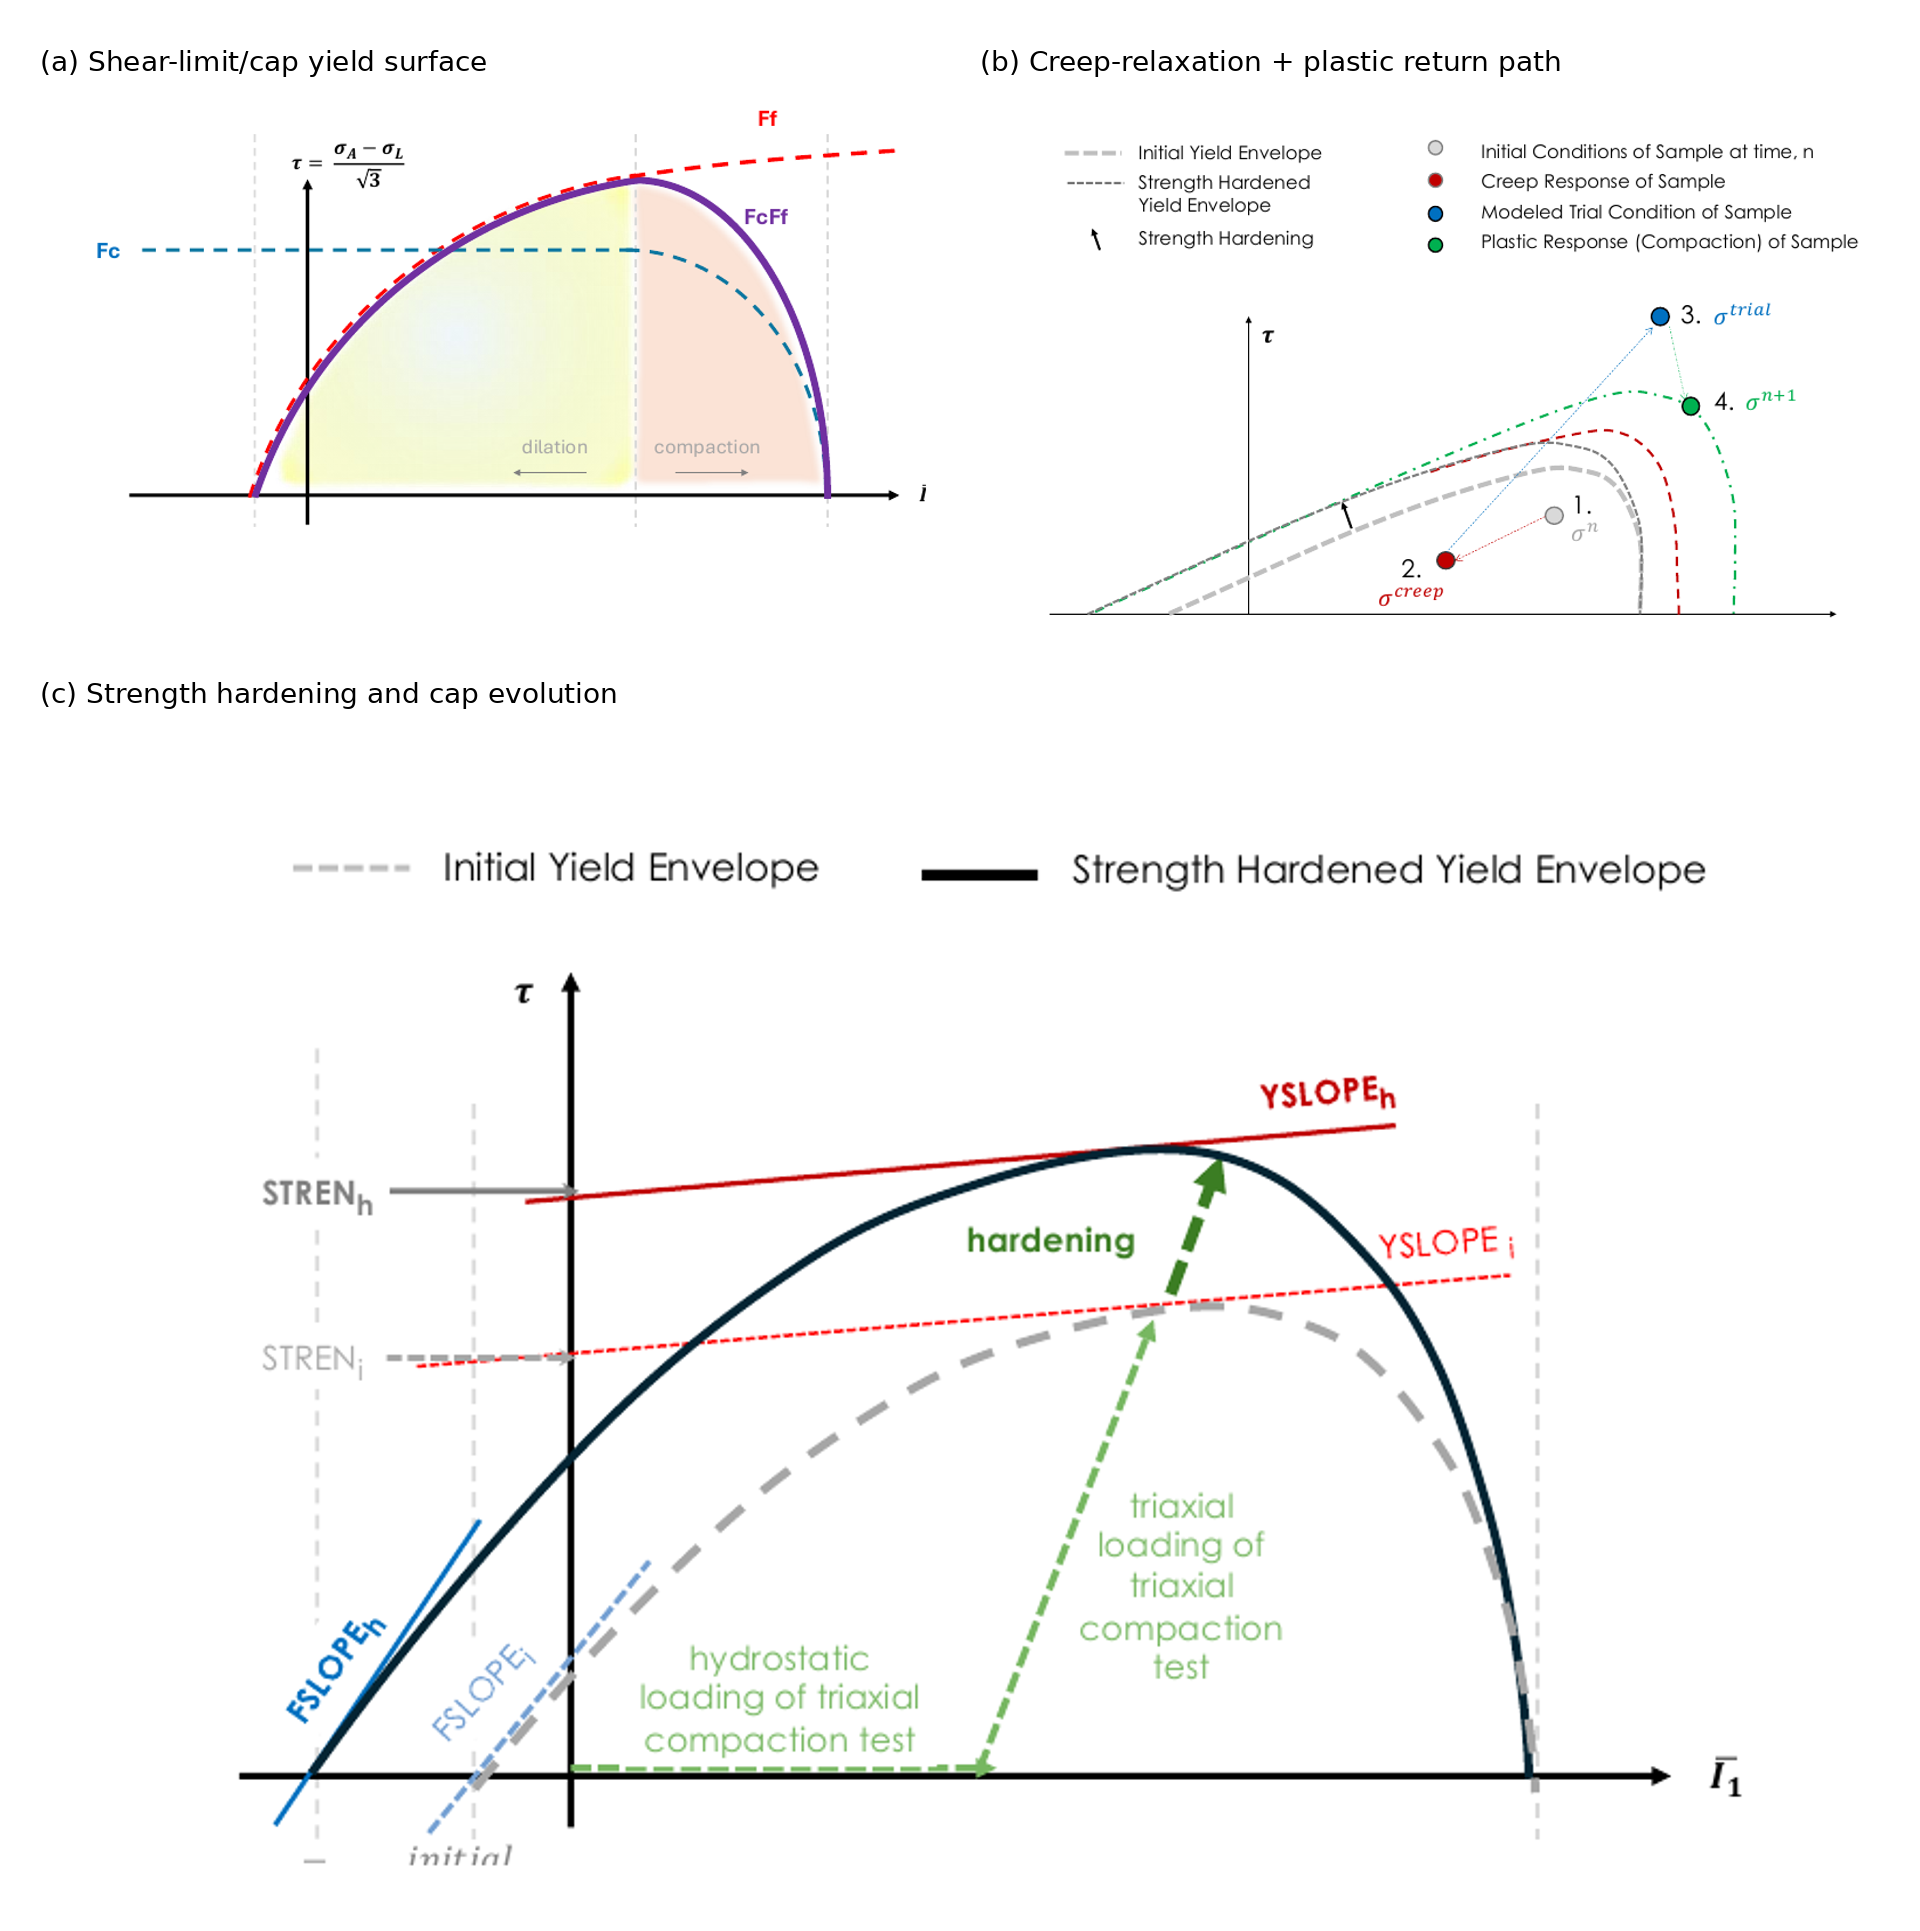
\includegraphics[width=0.98\linewidth]{figures/geomechanics_formulation_composite.png}
  \caption{Geomechanics formulation diagrams adapted from Malenda, Homel, Kibikas, Choens, Shalev, and Lyakhovsky~\cite{malenda2025ghareb}.  (a) The shear-limit function is multiplied by a cap function to obtain a pressure-sensitive strength surface.  (b) Creep first relaxes the beginning-of-step state, then an elastic trial stress is computed, and a plastic return is performed to the evolved surface.  (c) Strain hardening expands the strength envelope and shifts the triaxial-loading response.}
  \label{fig:geomechanics-formulation}
\end{figure}

\paragraph{Supported shear-limit parameterizations.}
The same input fields can represent several useful pressure-dependent limits.  The host-side input checks enforce a valid combination.
\begin{longtable}{@{}p{0.24\linewidth}p{0.68\linewidth}@{}}
\caption{Shear-limit surface families selected by \texttt{Geomechanics} inputs.\label{tab:geomechanics-surface-families}}\\
\toprule
\textbf{Family} & \textbf{Input pattern and purpose}\\
\midrule
\endfirsthead
\toprule
\textbf{Family} & \textbf{Input pattern and purpose}\\
\midrule
\endhead
Linear Drucker--Prager & \texttt{fSlope > 0}, \texttt{peakI1 >= 0}, and \texttt{stren = ySlope = 0}.  This gives a linear pressure-dependent shear limit.\\
Von Mises & \texttt{stren > 0} with \texttt{fSlope = peakI1 = ySlope = 0}.  This gives pressure-independent shear strength.\\
Zero-vertex transition & \texttt{fSlope > 0}, \texttt{stren > 0}, and \texttt{peakI1 = ySlope = 0}.  This connects a zero-pressure vertex to a finite shear plateau.\\
Nonlinear Drucker--Prager & \texttt{fSlope > ySlope > 0}, \texttt{stren > ySlope*peakI1}, and \texttt{peakI1 >= 0}.  This is the full curved form used for many geomaterial fits.\\
\bottomrule
\end{longtable}

For the nonlinear branch, the code computes
\begin{align}
  a_1 &= \texttt{STREN}_h, \\
  a_2 &= \frac{\texttt{FSLOPE}_h-\texttt{YSLOPE}_h}{\texttt{STREN}_h-\texttt{YSLOPE}_h\,\texttt{PEAKI1}_h},\\
  a_3 &= \left(\texttt{STREN}_h-\texttt{YSLOPE}_h\,\texttt{PEAKI1}_h\right)
         \exp\left[-a_2\,\texttt{PEAKI1}_h\right],\\
  a_4 &= \texttt{YSLOPE}_h.
  \label{eq:geomechanics-limit-parameters}
\end{align}
The linear and special-case surfaces are obtained by setting the corresponding subset of \(a_i\) to zero, as described in Table~\ref{tab:geomechanics-surface-families}.

\paragraph{Nonlinear elasticity.}
The tangent bulk modulus is evaluated from the beginning-of-substep stress and volumetric plastic strain.  In the dry path used by the reviewed code,
\begin{equation}
  K = b_0 + b_1\exp\left(\frac{b_2}{I_1}\right) - b_3\exp\left(\frac{b_4}{\epsilon_v^p}\right),
  \qquad I_1<0, \quad \epsilon_v^p<0,
  \label{eq:geomechanics-bulk-modulus}
\end{equation}
with lower bound \(K\ge b_0\).  The tensile/low-pressure response uses \(K=b_0\).  The shear modulus defaults to \(G=g_0\).  If \texttt{g1} is nonzero, the model computes a pressure-dependent Poisson ratio,
\begin{equation}
  \nu = g_1 + g_2\exp\left(\frac{g_3}{I_1}\right), \qquad 0\le \nu < \frac{1}{2},
  \label{eq:geomechanics-poisson}
\end{equation}
then sets
\begin{equation}
  G = \max\left[g_0,\frac{3K(1-2\nu)}{2(1+\nu)}\right].
  \label{eq:geomechanics-shear-modulus}
\end{equation}
This is a pragmatic pressure-dependent tangent stiffness for fitting laboratory data; it is evaluated substep-by-substep so the trial predictor follows the local tangent response.

\paragraph{Cap hardening, porosity, and crush curve.}
The cap position \(X\) is computed from volumetric plastic strain \(\epsilon_v^p=\operatorname{tr}\boldsymbol{\epsilon}^p\).  The implemented dry crush curve is
\begin{equation}
  X(\epsilon_v^p)=
  \begin{cases}
    \dfrac{p_0p_1+\ln\left[(\epsilon_v^p+p_3)/p_3\right]}{p_1}, & \epsilon_v^p\le 0,\\[0.8em]
    p_0(1+\epsilon_v^p)^{1/(p_0p_1p_3)}, & \epsilon_v^p>0,
  \end{cases}
  \label{eq:geomechanics-crush-curve}
\end{equation}
where \texttt{p0 < 0}, \texttt{p1 > 0}, and \texttt{p3 > 0}.  If \(\epsilon_v^p\) approaches \(-p_3\), the cap is pushed to a very large compressive value so the material behaves as fully compacted.  The particle porosity stored for plotting and subsequent material response is
\begin{equation}
  \phi = 1 + \exp(-\epsilon_v^p)(\phi_i-1),
  \qquad
  \phi_i = 1-\exp(-p_3).
  \label{eq:geomechanics-porosity}
\end{equation}
Thus the same input \texttt{p3} sets the limiting volumetric plastic compaction and the initial unloaded porosity implied by the crush curve.

\paragraph{Strain hardening and damage softening.}
The equivalent plastic shear strain is computed from the plastic-strain deviator.  When \texttt{strainHardeningK > 0}, the hardening increment is
\begin{equation}
  H = K_h\left(1-\exp[-n_h\,\bar\epsilon_p]\right),
  \label{eq:geomechanics-hardening}
\end{equation}
where \(K_h=\texttt{strainHardeningK}\) and \(n_h=\texttt{strainHardeningN}\).  The coherence \(c=1-D\) softens the surface through \(c^\psi\), where \(\psi=\texttt{fractureSofteningExponent}\).  In implementation form,
\begin{align}
  \texttt{STREN}_h &= b_{\mathrm{buckling}}\left(\texttt{stren}+H\,\texttt{dstrendh}\right),\\
  \texttt{FSLOPE}_h &= c^\psi\,\texttt{fSlope}\left(1+H\,\texttt{dfslopedh}\right)
  +\left(1-c^\psi\right)\texttt{fSlopeFailed},\\
  \texttt{PEAKI1}_h &= b_{\mathrm{buckling}}\left(\texttt{peakI1}+H\,\texttt{dpeakI1dh}\right)c^\psi s_p,\\
  c_{r,h} &= \operatorname{clamp}\left[\texttt{cr}\left(1+H\,\texttt{dcrdh}/g_0\right),10^{-10},0.99999999999\right],
  \label{eq:geomechanics-hardening-parameters}
\end{align}
where \(s_p\) is the particle \texttt{strengthScale}.  In this model, \texttt{strengthScale} is applied to the tensile-vertex/\texttt{peakI1} branch and to the fracture-stress threshold; it should not be assumed to scale every coefficient identically.  See Section~\ref{subsubsec:strength-scale-weibull} for the shared Weibull-strength discussion.

Damage is optional and active only when \texttt{fractureEnergyReleaseRate} is positive.  The model stores damage as \(D=1-c\).  Depending on \texttt{damageEvolutionCriterion}, damage increments are driven by dilatational plastic work or by a combined dilatational/shear plastic-work measure below a brittle--ductile transition pressure.  In schematic form,
\begin{equation}
  \Delta D = \frac{\Delta W_p\,\ell_{ch}}{G_f}, \qquad
  c^{n+1}=\max(0,c^n-\Delta D),
  \label{eq:geomechanics-damage}
\end{equation}
where \(G_f=\texttt{fractureEnergyReleaseRate}\) and \(\ell_{ch}\) is the particle length scale.  The damage threshold uses \texttt{fractureStress*strengthScale}; this is another model-specific use of \texttt{strengthScale}.  The \texttt{damageEvolutionCriterion=2} branch estimates the brittle--ductile transition from the apex of the current surface, while \texttt{damageEvolutionCriterion=1} uses the user-provided \texttt{brittleDuctileTransition}.

\paragraph{Optional creep relaxation.}
When \texttt{enableCreep=1}, creep is applied once over the full explicit time increment before the plastic substep retry loop.  The code uses an Arrhenius-like temperature multiplier
\begin{equation}
  A_T = \exp\left[-\frac{Q}{R}\left(\frac{1}{T}-\frac{1}{T_0}\right)\right],
  \label{eq:geomechanics-temperature-creep}
\end{equation}
where \(Q=\texttt{Q}\), \(T_0=\texttt{initialTemperature}\), and \(R\) is the gas constant.  Deviatoric creep uses an equilibrium plastic shear strain and relaxes the deviatoric stress toward it:
\begin{align}
  \gamma_{eq} &= C_0\,\tau^{C_1},\\
  \Delta\gamma_c &= \Delta t\,A_T C_2\max(\gamma_{eq}-\gamma_p,0),
  \label{eq:geomechanics-dev-creep}
\end{align}
with \(C_0=\texttt{creepC0}\), \(C_1=\texttt{creepC1}\), and \(C_2=\texttt{creepC2}\).  The increment is limited by the current elastic shear strain so creep cannot reverse the deviatoric stress in one step.

Volumetric creep uses the current unloaded porosity \(\phi_p\), an equilibrium porosity \(\phi_e\), and a pressure-dependent rate:
\begin{align}
  \phi_e &= \texttt{creepA}\exp\left[-\left(\frac{p}{\texttt{creepB}}\right)^{\texttt{creepD}}\right]
           + \texttt{creepE} - 0.0002\langle T-T_0\rangle - 3\times 10^{-6}\langle T-T_0\rangle^2,\\
  \frac{d\phi_p}{dt} &= -A_T\left(\frac{p}{\texttt{creepG}}\right)^{\texttt{creepF}}
  \texttt{creepC}\left(\phi_p-\phi_e\right),
  \label{eq:geomechanics-vol-creep}
\end{align}
where \(\langle x\rangle=\max(x,0)\).  The creep-updated porosity is converted back to an equivalent volumetric plastic strain and used to relax the beginning-of-step pressure.  As in the Ghareb-chalk implementation, the creep relaxation is intended to represent slow mechanisms in an explicit-dynamics calculation only when creep time scales are separated from elastic-wave and plastic-return time scales~\cite{malenda2025ghareb}.

\paragraph{Optional compaction/buckling multiplier.}
For porous or architected solids, \texttt{enableBuckling} applies a prescribed strength multiplier before the cap/plastic update.  With \texttt{enableBuckling=1}, the strain measure is volumetric, based on \(J=\det\mathbf{F}\).  With \texttt{enableBuckling=2}, the strain measure is directional, based on the stretch along \texttt{MaterialDirection}.  The multiplier has the form
\begin{equation}
  b_{\mathrm{buckling}} = 1-A_b\sin^2\left[-\left\lceil\frac{\ell_{ch}}{L_b}\right\rceil\pi\hat\epsilon\right],
  \label{eq:geomechanics-buckling}
\end{equation}
where \(A_b=\texttt{bucklingAmplitude}\), \(L_b=\texttt{bucklingLength}\), and \(\hat\epsilon\) is a normalized compaction strain.  This is an empirical multiplier, not a resolved structural-buckling analysis.

\paragraph{Numerical update algorithm.}
The GEOS-MPM call path is corotational.  The velocity gradient is unrotated into the beginning-of-step frame, symmetrized to form the strain-rate tensor, and the old plastic strain is also unrotated.  The model then performs the update in that frame and rotates the plastic strain back at the end of the step.

\begin{lstlisting}[caption={Geomechanics update structure.},label={alg:geomechanics-update},basicstyle=\ttfamily\small]
unrotate velocity gradient and plastic strain to beginning-of-step frame
D = sym(L_unrotated)
compute optional buckling multiplier from F and MaterialDirection
compute tangent K, G and conservative wave speed
if inelasticity is disabled:
  sigma = sigma_old + [3 K iso(D) + 2 G dev(D)] dt
else:
  estimate required substeps from trial stress and tangent-stiffness change
  apply optional full-step creep relaxation to sigma_old, ep_old, and X
  for progressively refined subcycle attempts:
    for each substep:
      evaluate K, G from current stress and plastic strain
      sigma_trial = hypoelastic predictor
      compute hardening, damage-modified surface coefficients, and yield state
      if elastic: accept trial state
      else:
        compute nonhardening return by transformed bisection/search
        if cap or backstress evolves:
          solve consistency on volumetric plastic strain by bounded bisection
        update plastic strain, cap X, coherence c, and porosity
    if all substeps succeed: accept attempt
  if all attempts fail: restore state and set constitutiveUpdateFlag = -1
rotate plastic strain back to end-of-step frame and store stress, damage, porosity
\end{lstlisting}

The nonhardening return uses the CB-TSCPR idea: transform the stress space so the energy-norm return becomes a Euclidean closest-point search, use bisection from an interior point to the trial point, and rotate the candidate point in transformed space until the closest boundary point is found~\cite{homel2015cbtscpr}.  The nonassociativity parameter \texttt{beta} enters this transformation by scaling the deviatoric coordinate,
\begin{equation}
  r^* = \beta\sqrt{\frac{3K}{2G}}\,r,
  \qquad r=\sqrt{2J_2},
  \label{eq:geomechanics-transformed-space}
\end{equation}
so the return direction can represent reduced or enhanced dilatation without constructing a separate flow-potential surface.  If the cap position changes with volumetric plastic strain, the solver wraps this return in a consistency bisection on \(\eta\in[0,1]\), where
\begin{equation}
  \Delta\epsilon_v^p = \eta\,\Delta\epsilon_{v,0}^p.
  \label{eq:geomechanics-consistency-eta}
\end{equation}
Each trial \(\eta\) updates \(X\), coherence, and the shifted-stress state, recomputes the return, and checks that the computed volumetric plastic strain matches the assumed value.  This decoupling is the main numerical reason the model can combine nonlinear elasticity, cap hardening, softening, and nonassociativity while retaining a robust update path.

\paragraph{Input parameterization.}
Table~\ref{tab:geomechanics-parameters} summarizes the major input groups.  The recommended calibration workflow is to fit \texttt{b0--b4} and \texttt{p0,p1,p3} from hydrostatic loading/unloading, fit \texttt{g0--g3}, \texttt{peakI1}, \texttt{fSlope}, \texttt{stren}, and \texttt{ySlope} from triaxial compression/extension data, then fit \texttt{strainHardeningK}, \texttt{strainHardeningN}, damage, and creep parameters from post-yield, dilation, compaction, and creep histories.

\begin{longtable}{@{}p{0.22\linewidth}p{0.28\linewidth}p{0.42\linewidth}@{}}
\caption{Main \texttt{Geomechanics} input groups.  See the generated schema appendix for the exact XML registration status and defaults.\label{tab:geomechanics-parameters}}\\
\toprule
\textbf{Group} & \textbf{Inputs} & \textbf{Role}\\
\midrule
\endfirsthead
\toprule
\textbf{Group} & \textbf{Inputs} & \textbf{Role}\\
\midrule
\endhead
Elasticity & \texttt{b0,b1,b2,b3,b4}, \texttt{g0,g1,g2,g3,g4} & Nonlinear tangent bulk modulus, pressure-dependent Poisson ratio, shear modulus, and conservative wave-speed estimate.  \texttt{g4} is registered but not active in the reviewed update path.\\
Cap/crush curve & \texttt{p0,p1,p2,p3,p4}, \texttt{cr} & Hydrostatic compaction curve, initial porosity relation, cap position, and cap branch point.  \texttt{p2} and \texttt{p4} are registered but currently unused.\\
Shear limit & \texttt{peakI1}, \texttt{fSlope}, \texttt{fSlopeFailed}, \texttt{stren}, \texttt{ySlope}, \texttt{beta} & Drucker--Prager/Kayenta-style shear surface, residual frictional slope, tensile vertex, and transformed-space nonassociativity.\\
Hardening & \texttt{strainHardeningK}, \texttt{strainHardeningN}, \texttt{dstrendh}, \texttt{dfslopedh}, \texttt{dpeakI1dh}, \texttt{dcrdh} & Exponential shear hardening and model-specific changes to strength, slope, tensile vertex, and cap branch.\\
Damage & \texttt{fractureEnergyReleaseRate}, \texttt{fractureSofteningExponent}, \texttt{fractureStress}, \texttt{brittleDuctileTransition}, \texttt{damageEvolutionCriterion} & Optional work-regularized reduction of coherence, with either user-specified or internally estimated brittle--ductile transition.\\
Creep and temperature & \texttt{enableCreep}, \texttt{creepC0}, \texttt{creepC1}, \texttt{creepC2}, \texttt{creepA}, \texttt{creepB}, \texttt{creepC}, \texttt{creepD}, \texttt{creepE}, \texttt{creepF}, \texttt{creepG}, \texttt{initialTemperature}, \texttt{Q} & Optional volumetric and deviatoric creep relaxation and temperature-scaled rates.\\
Buckling multiplier & \texttt{enableBuckling}, \texttt{bucklingLength}, \texttt{bucklingAmplitude}, \texttt{MaterialDirection} & Optional empirical compaction multiplier using volumetric or directional strain.\\
Numerical controls & \texttt{plasticStrainTolerance}, \texttt{stressReturnTolerance}, \texttt{maxAllowedSubcycles}, \texttt{failedStepResponse}, \texttt{disableInelasticity} & Return tolerances, subcycling limits, failure response, and elastic-only test mode.  Failed convergence exposes \texttt{constitutiveUpdateFlag=-1} to the solver robustness/deletion path.\\
Currently disabled fluid path & \texttt{fluidBulkModulus}, \texttt{fluidInitialPressure} & Must be zero in the reviewed implementation.  The code retains placeholders for a future persistent pore-pressure/backstress state.\\
\bottomrule
\end{longtable}

\paragraph{Implementation notes.}
The model writes \texttt{bulkModulus}, \texttt{shearModulus}, \texttt{porosity}, \texttt{damage}, \texttt{temperature}, and \texttt{constitutiveUpdateFlag} fields.  The stored \texttt{porosity} is an evolving continuum porosity inferred from volumetric plastic strain, not merely a visualization flag.  The stored \texttt{constitutiveUpdateFlag} is zero for normal updates, may be one when the model needed additional subcycling, and is set to \(-1\) when the update fails and the solver should treat the particle through the robustness/deletion logic in Section~\ref{sec:robustness-controls}.  The implementation is presently a dry porous solid model with optional empirical creep; coupled heat transfer, active fluid pressure, and fully coupled pore-pressure/backstress evolution are future extensions rather than active input options.


\subsection{Fluid models}
\label{subsec:fluid-constitutive-models}
\index{constitutiveModels!fluid models}

The reviewed MPM continuum dispatch includes a gas-like continuum model.  The PFW and XML infrastructure can assign this model to particles in the same way as solid models, but its stress is purely spherical.  A future liquid model can use the same dispatch path once implemented.

\subsubsection{\texttt{Gas}}
\label{subsubsec:gas-model}
\index{constitutiveModels!Gas}
\index{gas model}

\texttt{Gas} is a simple ideal-gas-style pressure model.  It computes a pressure from the reference pressure, the deformation-gradient Jacobian, and a temperature ratio, then returns a spherical compressive stress:
\begin{equation}
  p = \frac{p_0}{J}\frac{T}{T_0},
  \qquad
  \boldsymbol{\sigma}=-p\mathbf{I}.
  \label{eq:gas-pressure}
\end{equation}
The wave speed is evaluated as
\begin{equation}
  c = \sqrt{\gamma p/\rho},
  \qquad \gamma=1.4
  \label{eq:gas-wavespeed}
\end{equation}
for the current implementation.

\begin{lstlisting}[caption={Gas stress update.},label={alg:gas-update},basicstyle=\ttfamily\small]
pressure = referencePressure / jacobian * (temperature / referenceTemperature)
stress = -pressure * I
waveSpeed = sqrt(1.4 * pressure / density)
\end{lstlisting}

The gas model has special handling in the robustness/deformation-gradient-reset path (Section~\ref{sec:robustness-controls}) because a gas particle does not require the same persistent deviatoric deformation history as a solid particle.

\subsubsection{Liquid-model placeholder}
\label{subsubsec:liquid-model-placeholder}
\index{constitutiveModels!liquid placeholder}

A liquid-particle model is not currently documented as an active MPM continuum model in the reviewed snapshot.  A future liquid model could be introduced through the same material dispatch interface, for example with a weakly compressible equation of state,
\begin{equation}
  p = p_0 + K_f\left(\frac{\rho}{\rho_0}-1\right),
  \qquad
  \boldsymbol{\sigma}=-p\mathbf{I}+2\eta\operatorname{dev}\mathbf{D},
  \label{eq:liquid-placeholder}
\end{equation}
where \(K_f\) is a fluid bulk modulus and \(\eta\) is a dynamic viscosity.  This equation is a design placeholder only; it should not be interpreted as an implemented input option until a concrete GEOS-MPM liquid model is registered and verified.

\subsection{Shared constitutive modifiers and particle state}
\label{subsec:constitutive-modifiers}
\index{constitutive modifiers}

Several particle fields are not full constitutive models, but they modify how one or more models evaluate strength, damage, heat, or anisotropy.  These fields may be painted by geometry wrappers in PFW, updated by solver events, or updated by a constitutive model.  Because the same field may be interpreted differently by different models, this section documents the common data path and the expected modeling interpretation; model-specific equations should be added to the detailed material subsections before quantitative calibration.

\subsubsection{Strength scale and Weibull-type size effects}
\label{subsubsec:strength-scale-weibull}
\index{strengthScale}
\index{Weibull statistics}
\index{constitutive modifiers!strengthScale}

The particle field \texttt{strengthScale} is a multiplicative scalar that can be assigned by PFW geometry wrappers such as \texttt{strengthScaleWrapper} and by Voronoi/layered Weibull wrappers.  Models that expose a \texttt{strengthScale} wrapper then read the value during the constitutive update.  In brittle materials this field is often used to represent flaw-controlled size effects or mesoscopic heterogeneity.

A common theoretical basis is Weibull weakest-link scaling~\cite{weibull1951}.  For a reference volume \(V_0\), reference strength \(\sigma_0\), and Weibull modulus \(m\), the failure probability of a uniformly stressed volume \(V\) is often written
\begin{equation}
  P_f = 1 - \exp\left[-\frac{V}{V_0}\left(\frac{\sigma}{\sigma_0}\right)^m\right].
  \label{eq:weibull-failure-probability}
\end{equation}
At fixed failure probability this gives the familiar deterministic size scaling
\begin{equation}
  \sigma(V) = \sigma_0\left(\frac{V_0}{V}\right)^{1/m}.
  \label{eq:weibull-size-scaling}
\end{equation}
A stochastic PFW wrapper may instead sample a flaw population and assign a particle-level scale factor \(s_p\) so that the material model evaluates a local strength such as \(Y_p=s_pY_0\) or \(\sigma_{f,p}=s_p\sigma_f\).  The exact placement of \(s_p\) is model dependent: for example, some models multiply tensile and compressive strengths, some multiply fracture-energy parameters only when an option is enabled, and some models do not use the field at all.  For that reason, \texttt{strengthScale} should be documented in each detailed material subsection before it is used for quantitative calibration.

\subsubsection{Crack-tip stress concentration}
\label{subsubsec:crack-tip-stress-concentration}
\index{crack-tip stress concentration}
\index{distanceToCrackTip}
\index{constitutive modifiers!crack-tip correction}

The crack-tip correction is a solver/constitutive coupling used by damage models that need an unresolved stress-concentration estimate near a DFG fracture tip, motivated by the Griffith-Irwin crack-tip picture~\cite{griffith1921,irwin1957}.  The solver first uses the neighbor-list damage field to compute a nonlocal damage gradient and a local Hessian-like diagnostic.  Particles that satisfy the tip-detection threshold receive a positive \texttt{distanceToCrackTip}; other particles receive zero.  Models such as \texttt{CeramicDamage} and \texttt{Graphite} can then compute and store a plotted \texttt{crackTipStressConcentration} factor.

The current correction has the form
\begin{equation}
  C_{\mathrm{tip}}
  = \max\left(1,\sqrt{\frac{d_{\mathrm{tip}}}{r_{\mathrm{fpz}}}}\right),
  \label{eq:crack-tip-stress-concentration-outline}
\end{equation}
where \(d_{\mathrm{tip}}\) is the inverse-kernel estimate of the unresolved distance to the crack tip and \(r_{\mathrm{fpz}}\) is a process-zone length constructed from fracture toughness or fracture energy and a nominal intact strength.  The intent is to avoid over-predicting the resolved particle strength when the MPM/DFG length scale cannot resolve the near-tip stress field.  The correction is optional and should be verified against the intended fracture model and neighbor radius.

\subsubsection{Porosity}
\label{subsubsec:constitutive-porosity}
\index{porosity}
\index{constitutive modifiers!porosity}

\texttt{porosity} is a particle field that may be initialized by PFW, painted by wrappers such as \texttt{porosityWrapper} or \texttt{pointwisePorosityWrapper}, read by a constitutive model, and in some models updated as part of the material response.  In the reviewed code path, porous/damage models use porosity differently.  For example, \texttt{Geomechanics} carries porosity as an evolving material variable, while \texttt{CeramicDamage} uses porosity in strength scaling.  Solver events and future coupled solvers may also modify porosity, for example to represent healing, compaction, reaction, or pore closure.

Because porosity can be both an input descriptor and a constitutive state variable, users should distinguish the initial particle field from any model-updated value written after the first constitutive step.  Future coupled heat/fluid/chemistry or poromechanics updates should document ownership rules: whether the solver, a flow model, or the solid constitutive model is the authoritative updater for \texttt{porosity} at a given step.

\subsubsection{Temperature}
\label{subsubsec:constitutive-temperature}
\index{temperature}
\index{constitutive modifiers!temperature}
\index{TemperatureProfile event}
\index{TemperatureRamp event}

\texttt{temperature} and \texttt{temperatureRate} are particle fields shared by the solver, events, and thermally sensitive constitutive models.  PFW can initialize temperature through geometry wrappers, while events such as \texttt{TemperatureProfile} can prescribe domain-wide histories from an event-local table.  The reviewed code also records internal energy and includes constitutive hooks for temperature-dependent parameters.  Models such as \texttt{StrainHardeningPolymer}, \texttt{Graphite}, and \texttt{Geomechanics} read temperature-dependent terms; other models may ignore temperature unless later extended.

In a purely mechanical run, temperature may be prescribed externally or inferred internally by a constitutive model from plastic work, strain energy, or an equation of state.  In future coupled runs, a heat-transfer solver could become the authoritative updater.  Until those ownership rules are formalized for a given application, input files should make clear whether temperature is a fixed initial condition, an event-prescribed history, a material-model output, or a field reserved for later coupling.

\subsection{External material models}
\label{subsec:external-material-models}
\index{constitutiveModels!external material models}
\index{external material models}
\index{setupMPM!external material models}

GEOS-MPM can compile continuum material models that live outside the public source tree.  This path is intended for site-local, application-specific, or proprietary continuum laws without requiring those files to be committed to the main repository.  The build hook is the CMake cache variable \texttt{GEOS\_EXTERNAL\_CONSTITUTIVE\_MODELS\_DIR}; the \texttt{setupMPM} helper described in Section~\ref{sec:setupMPM} forwards this path through the option \texttt{--external-material-models}.

A minimal external material-model directory has the form
\begin{lstlisting}[caption={Minimal external material-model directory layout.},label={lst:external-material-layout},basicstyle=\ttfamily\small]
my_external_materials/
  GEOSExternalConstitutiveModels.cmake
  MyContinuumModel.hpp
  MyContinuumModel.cpp
\end{lstlisting}
The manifest can also be named \texttt{CMakeLists.txt}.  For an explicit MPM continuum model, the manifest must list the source/header files and must also add the model type and include to the MPM dispatch lists:
\begin{lstlisting}[caption={External continuum model CMake registration.},label={lst:external-material-cmake},basicstyle=\ttfamily\small]
geos_register_external_constitutive_models(
  BASE_DIR ${CMAKE_CURRENT_LIST_DIR}
  SOURCES
    MyContinuumModel.cpp
  HEADERS
    MyContinuumModel.hpp
  MPM_INCLUDES
    MyContinuumModel.hpp
  MPM_MODELS
    MyContinuumModel )
\end{lstlisting}
The implementation file must still register the model with the normal GEOS constitutive catalog, for example
\begin{lstlisting}[language=C++,caption={External model GEOS catalog registration.},label={lst:external-material-catalog},basicstyle=\ttfamily\small]
REGISTER_CATALOG_ENTRY( ConstitutiveBase,
                        MyContinuumModel,
                        std::string const &,
                        Group * const )
\end{lstlisting}
After the files are in place, configure and build using either the setup helper or a direct CMake configuration:
\begin{lstlisting}[language=bash,caption={Building with external continuum material models.},label={lst:external-material-build},basicstyle=\ttfamily\small]
./setupMPM --dane --external-material-models /path/to/my_external_materials

# Equivalent direct-CMake idea:
cmake -DGEOS_EXTERNAL_CONSTITUTIVE_MODELS_DIR=/path/to/my_external_materials ...
cmake --build <build-dir> --target geosx
\end{lstlisting}

Once built, the external material is used like any other continuum model: add a corresponding XML tag to the \texttt{Constitutive} block, add its name to the relevant \texttt{ParticleRegion} material list, and assign the matching material index with PFW geometry objects or wrappers.  External cohesive-zone laws use a related but separate registration list and are documented with the cohesive-zone infrastructure in Section~\ref{sec:cohesive-zone-implementation}.
